\section{Three-level system}\label{sec:pw3l}

A two-level system is the simplest non-trivial quantum system and,
as seen in Sec.~\ref{sec:absorption+pw},
it is sufficient to illustrate
models of quantum time of arrival,
such as those based on complex potentials,
as well as relational models.
Therein, numerical examples have been shown, where the two approaches
---discrete Page--Wootters and the ``non Hermitian'' detector models---
lead to
compatible predictions.

A three-level atom (or a three-level quantum system in general) appears
naturally
as
the next computational step;
but far from being merely another excercise
---just at a slightly higher level of complexity
but otherwise showing, essentially, the same physics---
it is in fact the \emph{minimal} system \emph{required}
to realize a broad
phenomenology that includes the
\term{Stimulated Raman adiabatic passage}
---STIRAP \parencite{Ruschhaupt_AtomDiode, NonHermitianShortcutSTIRAP, OptimizedTransferSTIRAP, Ruschhaupt_STA23}
and the
\term{Electromagnetically induced transparency}
---EIT \parencite{EIT_Review}.

Also, it wil be shown that a three-level atom can model
a more robust and realistic
detector for time-of-arrival measurement, compared to the one implemented
with a two-level atom (as introduced in Sec.~\ref{sec:hist:detect}).
The atom can be ``driven'' by a laser
from the ground state $\ket{0}$ into the excited state $\ket{2}$,
then decay into a metastable state $\ket{1}$ at an intermediate energy
(see the above references, although they might use a slightly different notation).
This prevents the atom from decaying again and altering the ``arrival'' detection.

As usual, we're going to set $\hbar = 1$ in the following numerical computation,
based, once again, on the
\emph{NumPy} framework \parencite{comp:numpy},
within a
\term{Jupyter notebook} \parencite{comp:jupyter}.
Details can be consulted in the Appendix~\ref{detector-model-3-level-system}.
Full source code is available from the repository at ref. \cite{OwnJupyterRepo}.

\subsection{Hermitian evolution}

In our numerical example, the following
Hamiltonian is considered:
\begin{equation}\label{eq:3lev:H}
  H \repr \frac{1}{96} \mqty(
    -2  & 0 & 32  \\
     0  & 2 & 8   \\
    32  & 8 & 3
  )
  \text{,}
\end{equation}
with respect to the fiducial basis $\qty{\ket{0}, \ket{1}, \ket{2}}$.
Let also
the initial state be $\ket{\psi(0)} = \ket{0} \repr \mqty(1 \\ 0 \\ 0)$.

The system will evolve \emph{unitarily}, according to $\ket{\psi(t)} = \E^{-\iu H t} \ket{\psi(0)}$,
which is computed numerically:
\begin{lstlisting}[language=Python]
import numpy as np
from scipy.linalg import expm, norm

H = np.array([
  [-2,     0,      32],
  [0,      2,       8],
  [32,     8,       3]
], np.complex_) / 96

psi_0 = np.array([1, 0, 0], np.complex_)

def U(t):
    return expm(-1j*H*t)

def unitary_psi(t):
    return U(t) @ psi_0
\end{lstlisting}

We're interested in the probability of the system to be in $\ket{0}$, $\ket{1}$, or $\ket{2}$,
which is given by $\abs{\braket{0, 1, 2}{\psi(t)}}^2$:
\begin{lstlisting}[language=Python]
def prob(t):
  probabilities = [0, 0, 0]
  for i in 0, 1, 2:
      probabilities[i] = norm(unitary_psi(t)[i])**2
      return probabilities
\end{lstlisting}
Such probabilities over time are shown in Figure \ref{fig:3lev:probs}. 

\begin{figure}[h]
  \begin{subfigure}[b]{\textwidth}
    \centering
    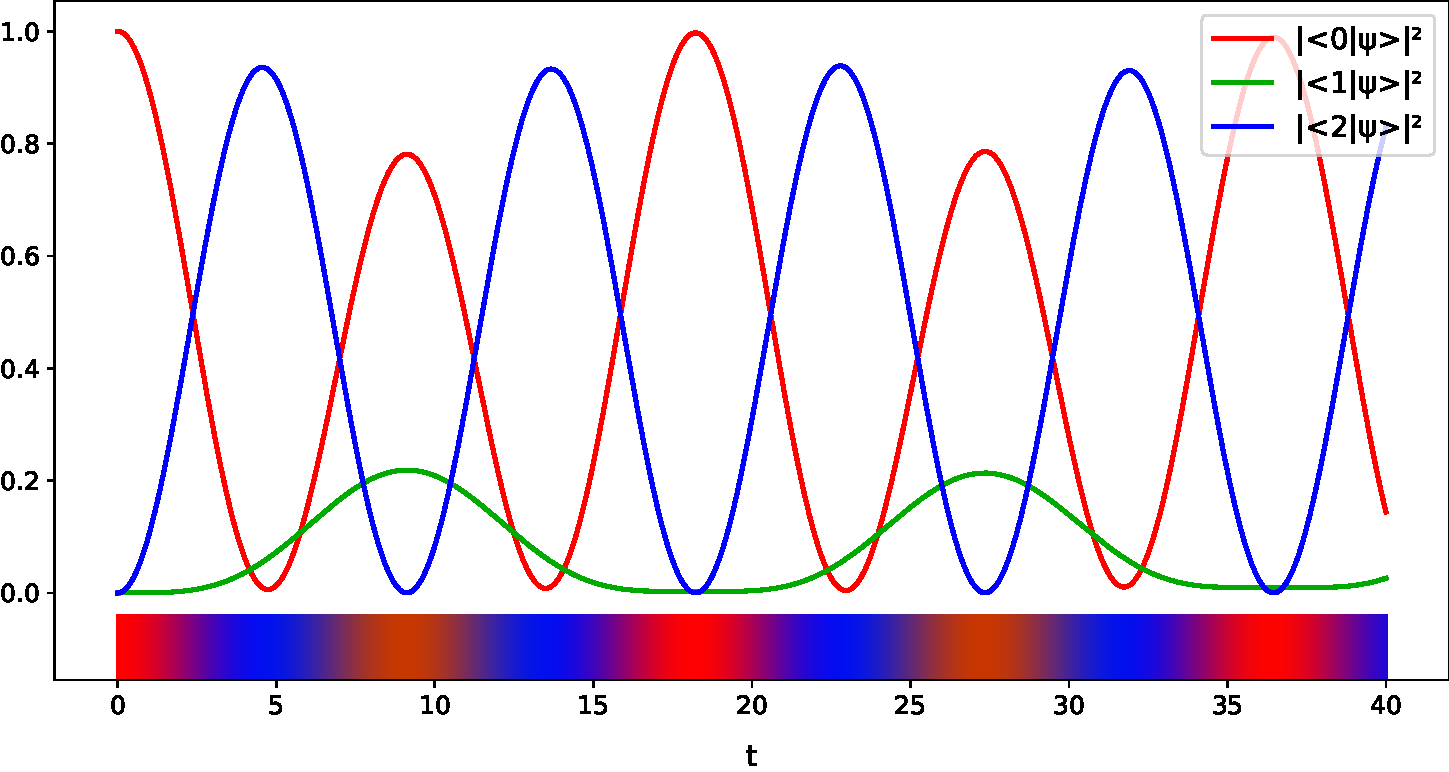
\includegraphics[width=.8\textwidth]{img/3ldetect/hermitian3lines.pdf}
    \subcaption{
      Probabilities for the three-level system.
      \emph{Note}:
        a three-level system allows a graphical representaion
        where primary colors can be combined
        (see the bar at the bottom) to immediately
        visualize which probability dominates.
    }
    \label{fig:3lev:probs:lines}
  \end{subfigure}
  \par\bigskip
  \par\bigskip
  \begin{subfigure}[b]{\textwidth}
    \centering
    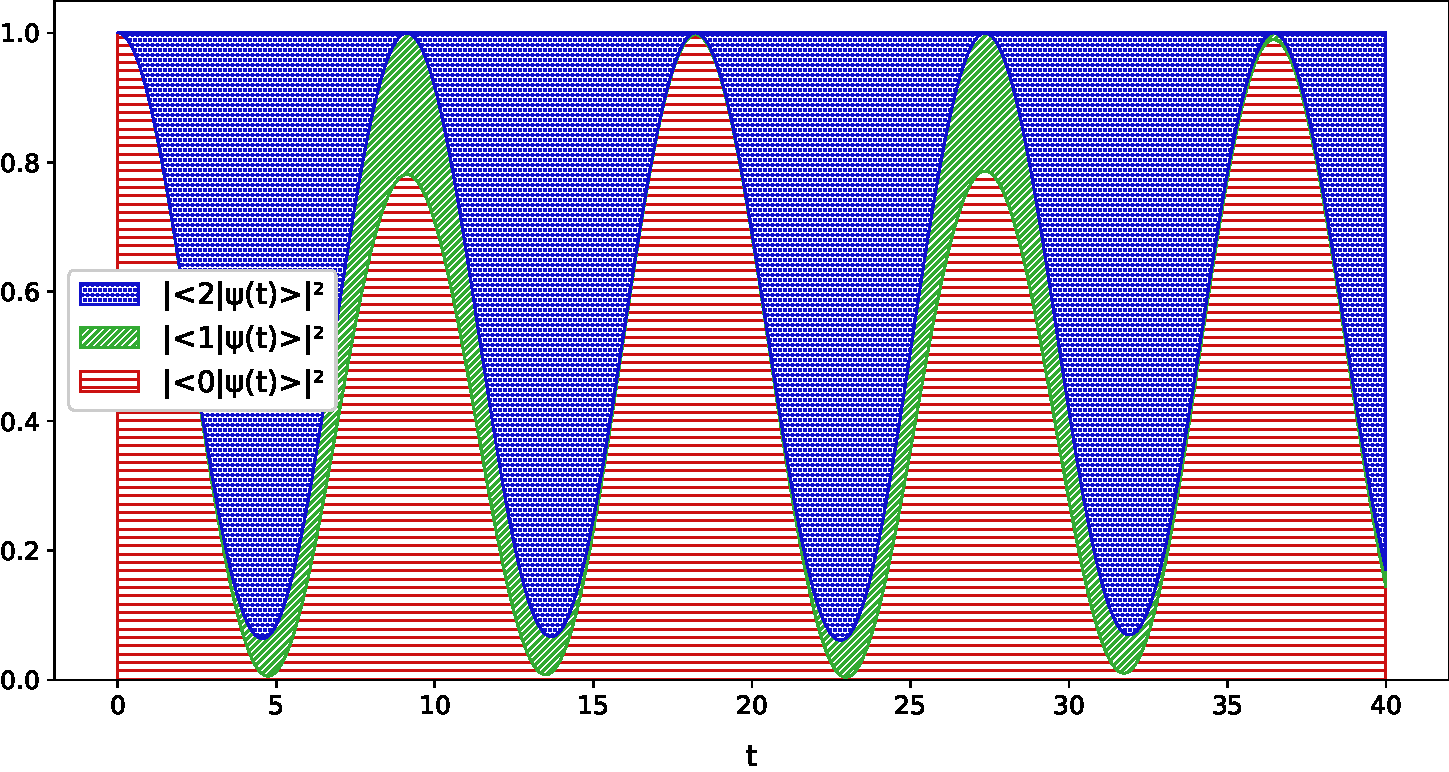
\includegraphics[width=.8\textwidth]{img/3ldetect/hermitian3color.pdf}
    \subcaption{\setstretch{1.25}
      \emph{Stacked} probability chart shows that their sum
      $\sum_{i=0}^{2} \abs{\braket{i}{\psi(t)}}^2$
      is constantly equal to 1 at any time $t$.
      That is equal to the norm $\norm{\psi(t)}^2$, which is indeed conserved
      as
      the system evolves \emph{unitarily}.
    }
    \label{fig:3lev:probs:stack}
  \end{subfigure}
  \par\bigskip
  \par\bigskip
  \caption{
    Probabilities
      $\abs{\braket{i}{\psi(t)}}^2$ for $i \in \qty{0, 1, 2}.$
  }
  \label{fig:3lev:probs}
\end{figure}

We are also interested in probability \term{amplitudes}:
complex values of
$\braket{0}{\psi(t)}$, 
$\braket{1}{\psi(t)}$, and
$\braket{2}{\psi(t)}$
are represented in the three-dimensional
plot in Fig.~\ref{fig:3lev:hermitianEvol}.
Once again, the two horizontal axes are used for the real and imaginary part of
$\braket{0, 1, 2}{\psi(t)}$,
while the independend variable $t$ (time) is represented on the vertical axis.
\begin{figure}[h]
  \begin{subfigure}[t]{\textwidth}
    \centering
    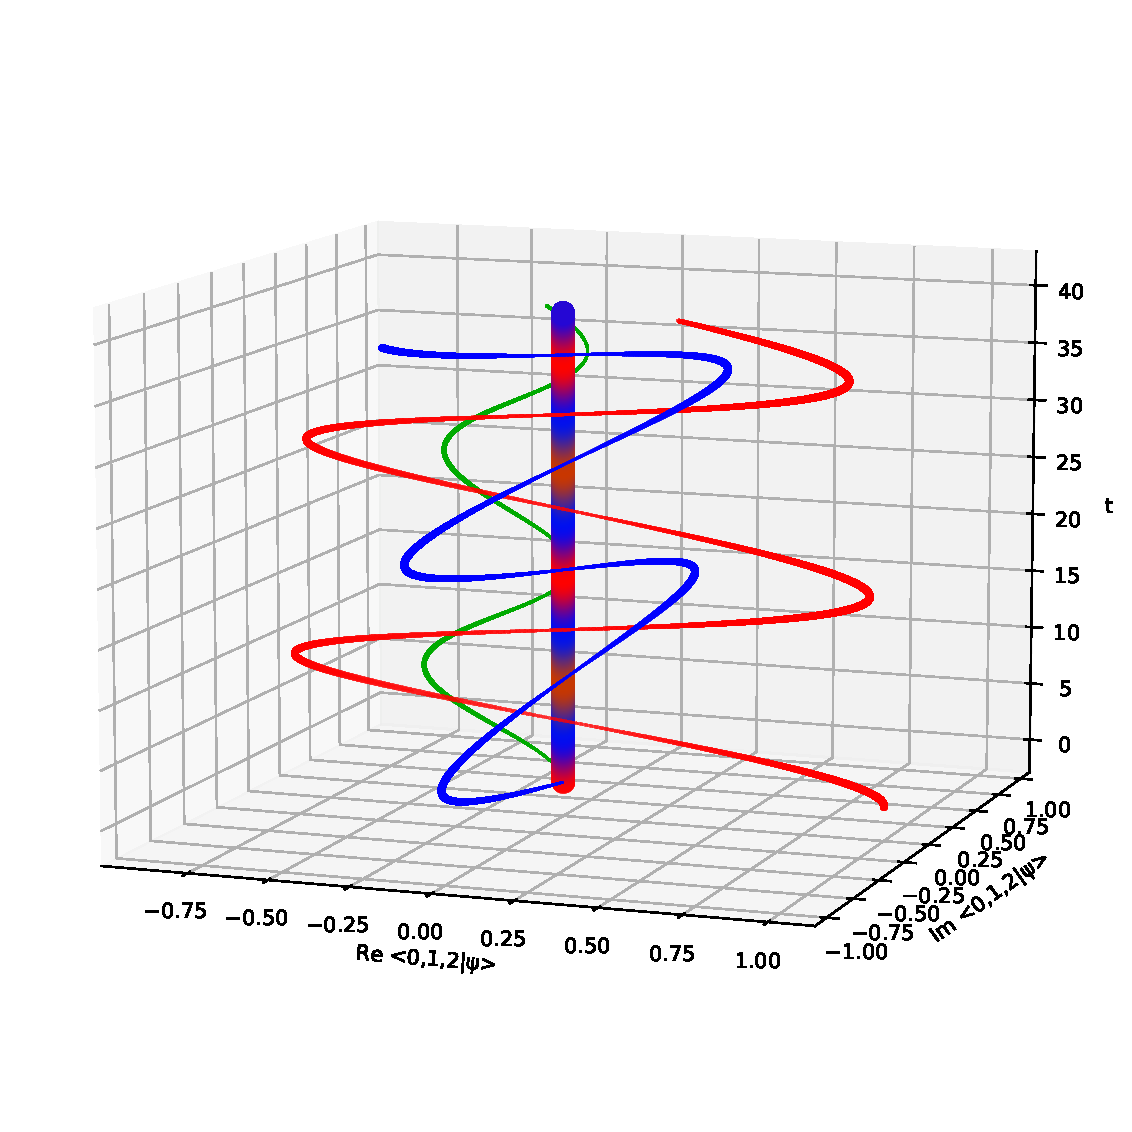
\includegraphics[height=0.45\textheight,clip,trim=80 180 40 140]{img/3ldetect/hermitianSpaceTime_side.pdf}
    \caption{``Side'' view.}
  \end{subfigure}
  \par\bigskip
  \begin{subfigure}[b]{\textwidth}
    \centering
    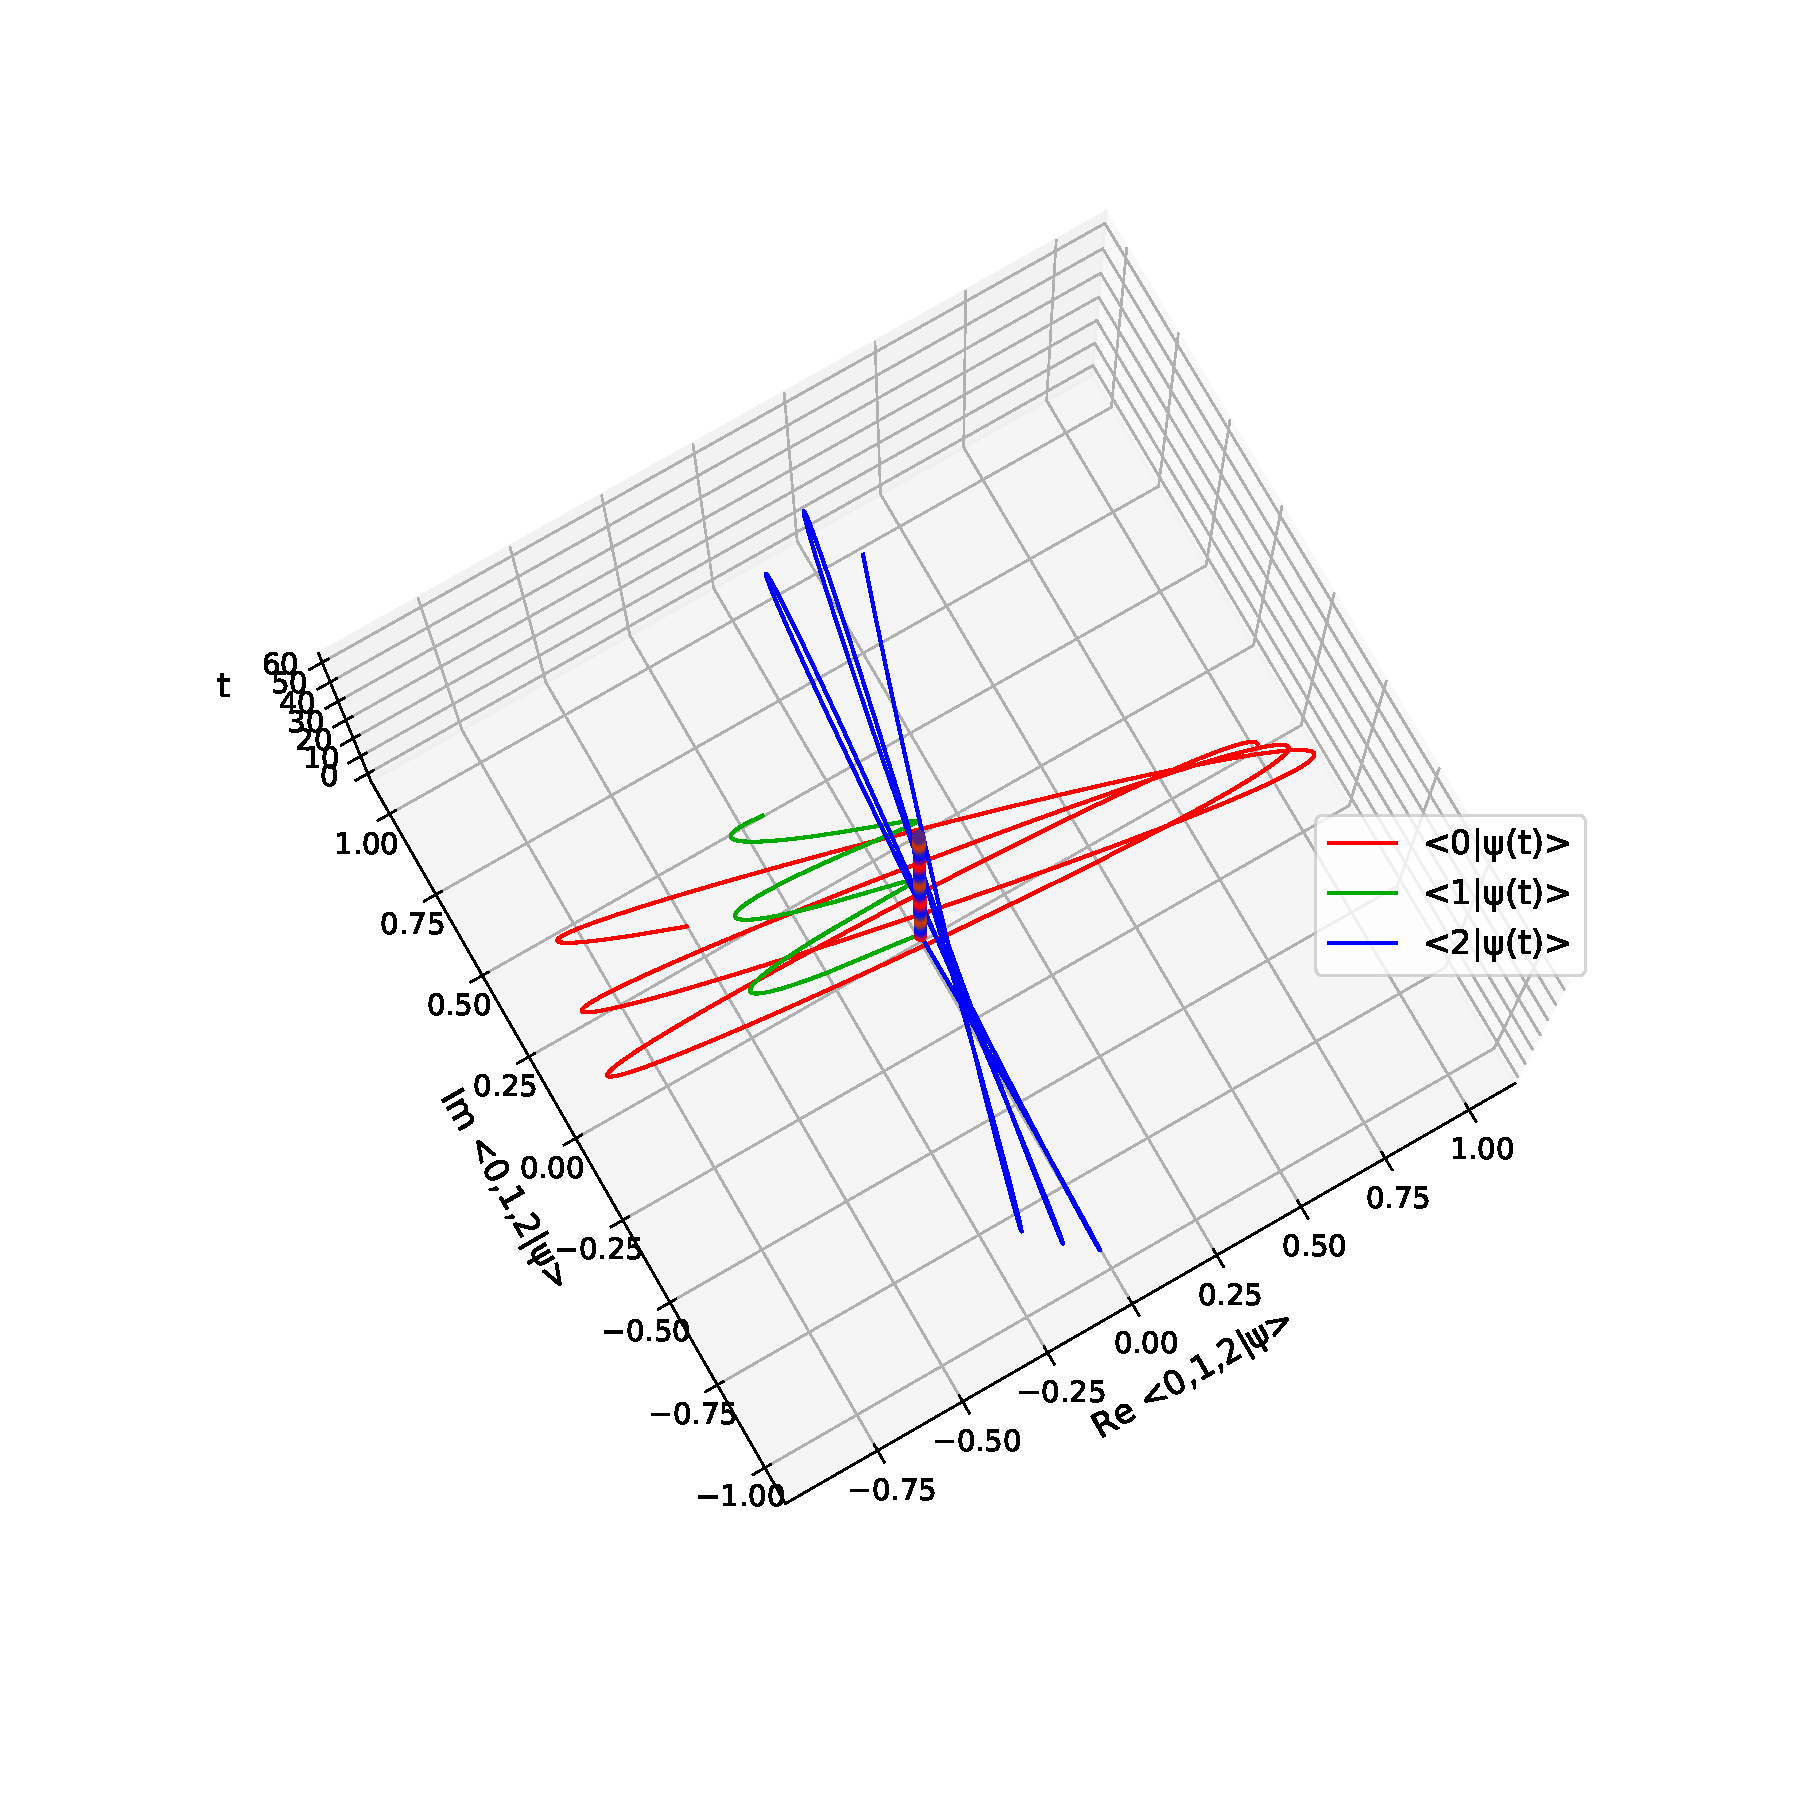
\includegraphics[height=0.41\textheight,clip,trim= 20 120 20 220]{img/3ldetect/hermitianSpaceTime_top.pdf}
    \caption{``Top'' view.}
  \end{subfigure}
  \caption{
    \textit{3-D plot} showing the complex values of the
    probability \emph{amplitudes} $\braket{0, 1, 2}{\psi(t)}$.
    Real and imaginary parts of those values are represented on
    the first two axes, while the independent variable (time, $t$)
    is represented
    on the third axis.
    -- Additionally, the vertical axis is coloured to encode \emph{probabilities}
    (absolute values)
    in a similar fashion to Fig. \ref{fig:3lev:probs:lines}. 
  }
  \label{fig:3lev:hermitianEvol}
\end{figure}

\subsection*{\textit{A note on graphical representation}}

Other than visualizing complex-valued functions with three-dimensional plots,
another visualization technique, utilized in various plots in this Section,
consists of leveraging
the fact that the system has exactly 3 levels,
thus allowing three primary colors, red, green and blue, to be combined
in proportion to the probabilities $\abs{\braket{i}{\psi(t)}}$
respectively for $i = 0, 1, 2$. This allows an immediate visualization
of which level, $\ket{0}$, $\ket{2}$ or $\ket{2}$, predominates statistically, if any.
To better clarify this with an example,
a snippet of the implemtation of Fig. \ref{fig:3lev:probs} follows.
\begin{lstlisting}[language=Python]
# [...]
import matplotlib
import matplotlib.pyplot as plt

# [...]
for i in 0, 1, 2:
  probs[i] = np.fromiter((prob(t)[i] for t in times), np.float)

# [...]
rgbs = []
for i in range(NPLOTPOINTS):
    rgbs.append(
        (
            probs[0][i],
            probs[1][i],
            probs[2][i]
        )
    )

# [...]
fig, ax = plt.subplots(figsize=(12,6))
ax.set_xlabel('t')
ax.scatter(times, np.zeros(NPLOTPOINTS)-0.1, c=rgbs, marker='|', s=400)
\end{lstlisting}


\subsection{Complex potential -- non-Hermitian evolution}

In a similar fashion to what seen in Section \ref{sec:hist:detect},
the Hermitian Hamiltonian $\hat{H}$, from eq.~\eqref{eq:3lev:H},
is replaced by
\begin{equation}\label{eq:3lev:nonUnitaryH}
  K \eqbydef \hat{H} - \iu \hat{D} \text{,}
\end{equation}
where
\begin{equation}\label{eq:3lev:nonUnitaryH:antiHermitianTerm}
  \hat{D} \repr \mqty(
    0 &0 &0 \\
    0 &0 &0 \\
    0 &0 &\gamma
  ) \text{.}
\end{equation}
This models the absorptive detection of the ``arrival'' of the system at state~$\ket{2}$.
A numeric value of $\gamma = \mathtt{0.1}$ is chosen for the current simulation.
Repeating the calculation for the time-evolution
brings to
probabilities, and probability amplitudes,
that are graphically visualized in Fig. \ref{fig:3lev:loss3color}, and \ref{fig:3lev:nonHermitianEvol},
and can be compared with the Hermitian (i.e. unitary) case,
Figs. \ref{fig:3lev:probs:stack} and \ref{fig:3lev:hermitianEvol} respectively.
It appears clearly, in Fig. \ref{fig:3lev:loss3color},
that the norm of the state vector is not
conserved, but decreases monotonically. 
%
\begin{figure}[h]
  \begin{subfigure}[b]{\textwidth}
    \centering
    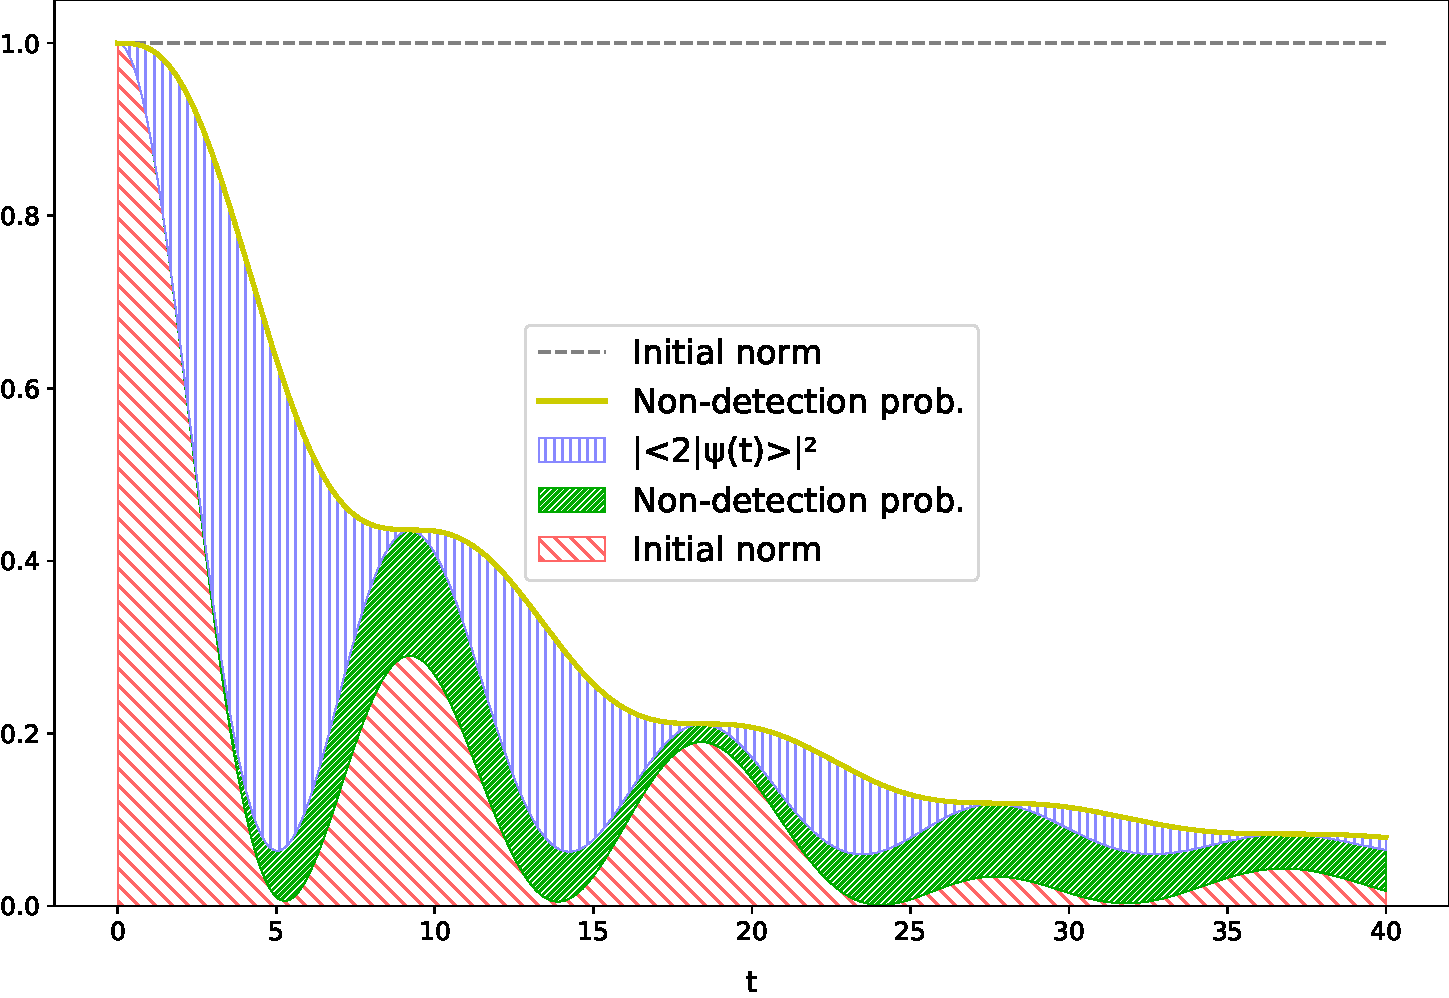
\includegraphics[width=.8\textwidth]{img/3ldetect/loss3color.pdf}
    \subcaption{\setstretch{1.33}
      \emph{Stacked} probability chart (non-Hermitian case) shows that norm
      $\norm{\psi(t)}^2 = \sum_{i=0}^{2} \abs{\braket{i}{\psi(t)}}^2$
      is monotonically decreasing. The actual state probabilities
      will need to be renormalized due to the norm loss of $\ket{\psi(t)}$.
    }
    \label{fig:3lev:loss3color}
  \end{subfigure}
  \par\bigskip
  \par\bigskip
  \begin{subfigure}[b]{\textwidth}
    \centering
    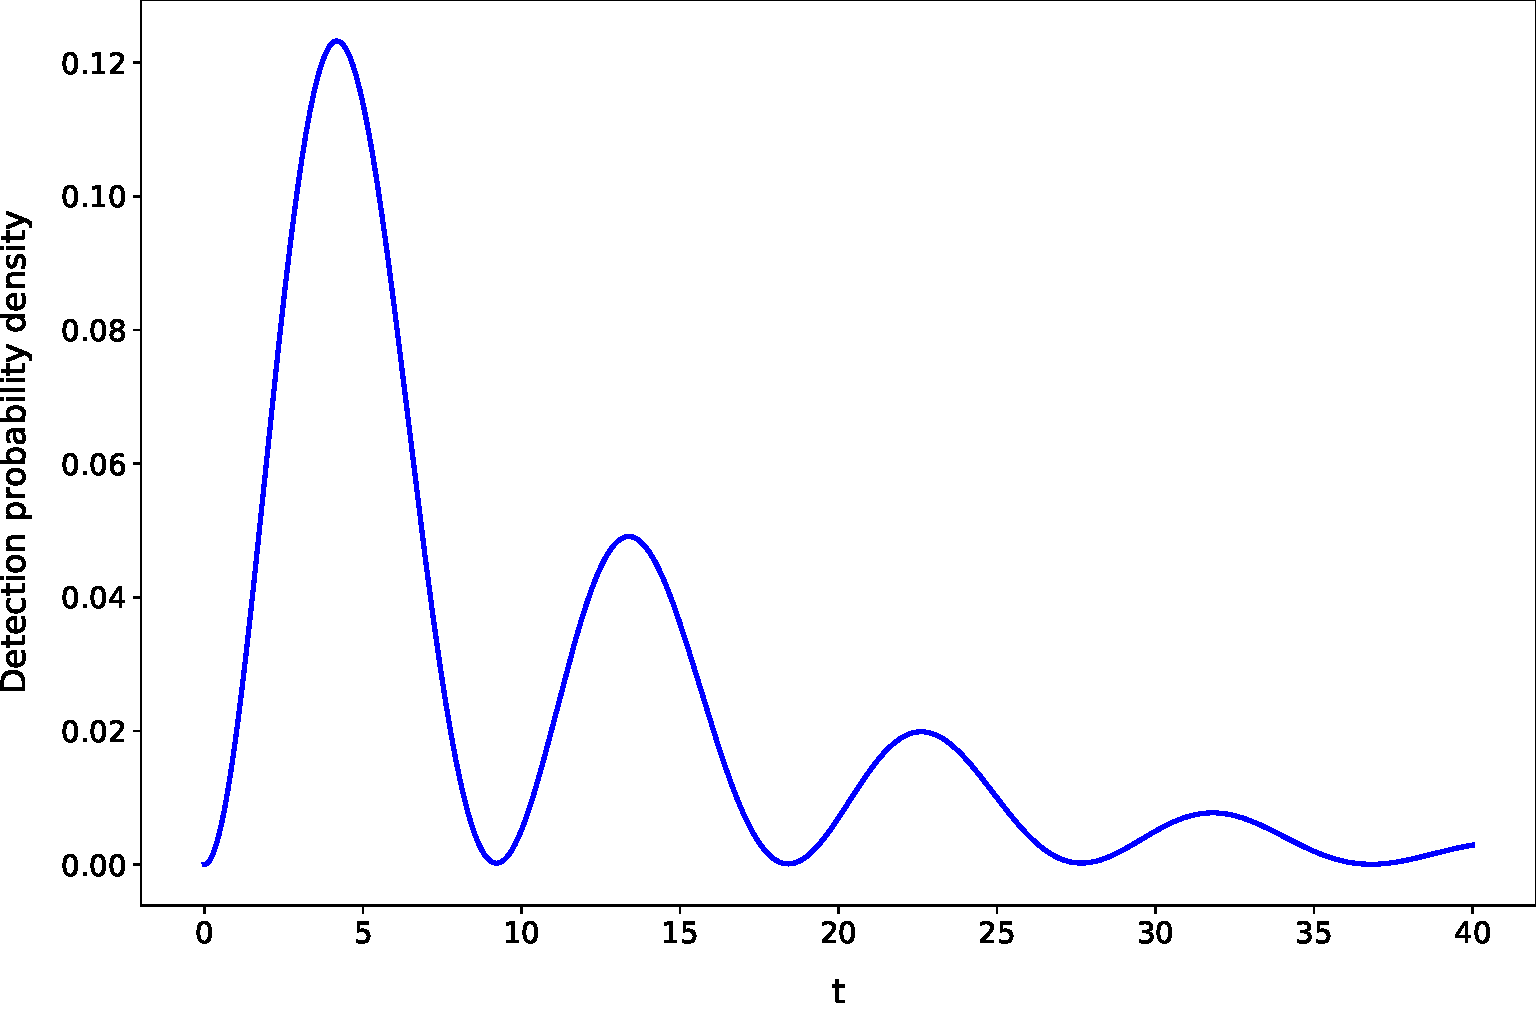
\includegraphics[width=.8\textwidth]{img/3ldetect/loss.pdf}
    \subcaption{
      Normalization loss rate $-\dv{\norm{\psi}^2}{t}$.
      Equates the time-of-arrival probability distribution (at the ``absorbing'' state $\ket{2}$).
    }
    \label{fig:3lev:loss}
  \end{subfigure}
  \par\bigskip
  \par\bigskip
  \caption{
    Absorptive detector model: norm loss and probabilities.
  }
  \label{fig:3lev:nonHermitianProbs}
\end{figure}
%
\begin{figure}[h]
  \begin{subfigure}[b]{\textwidth}
    \centering
    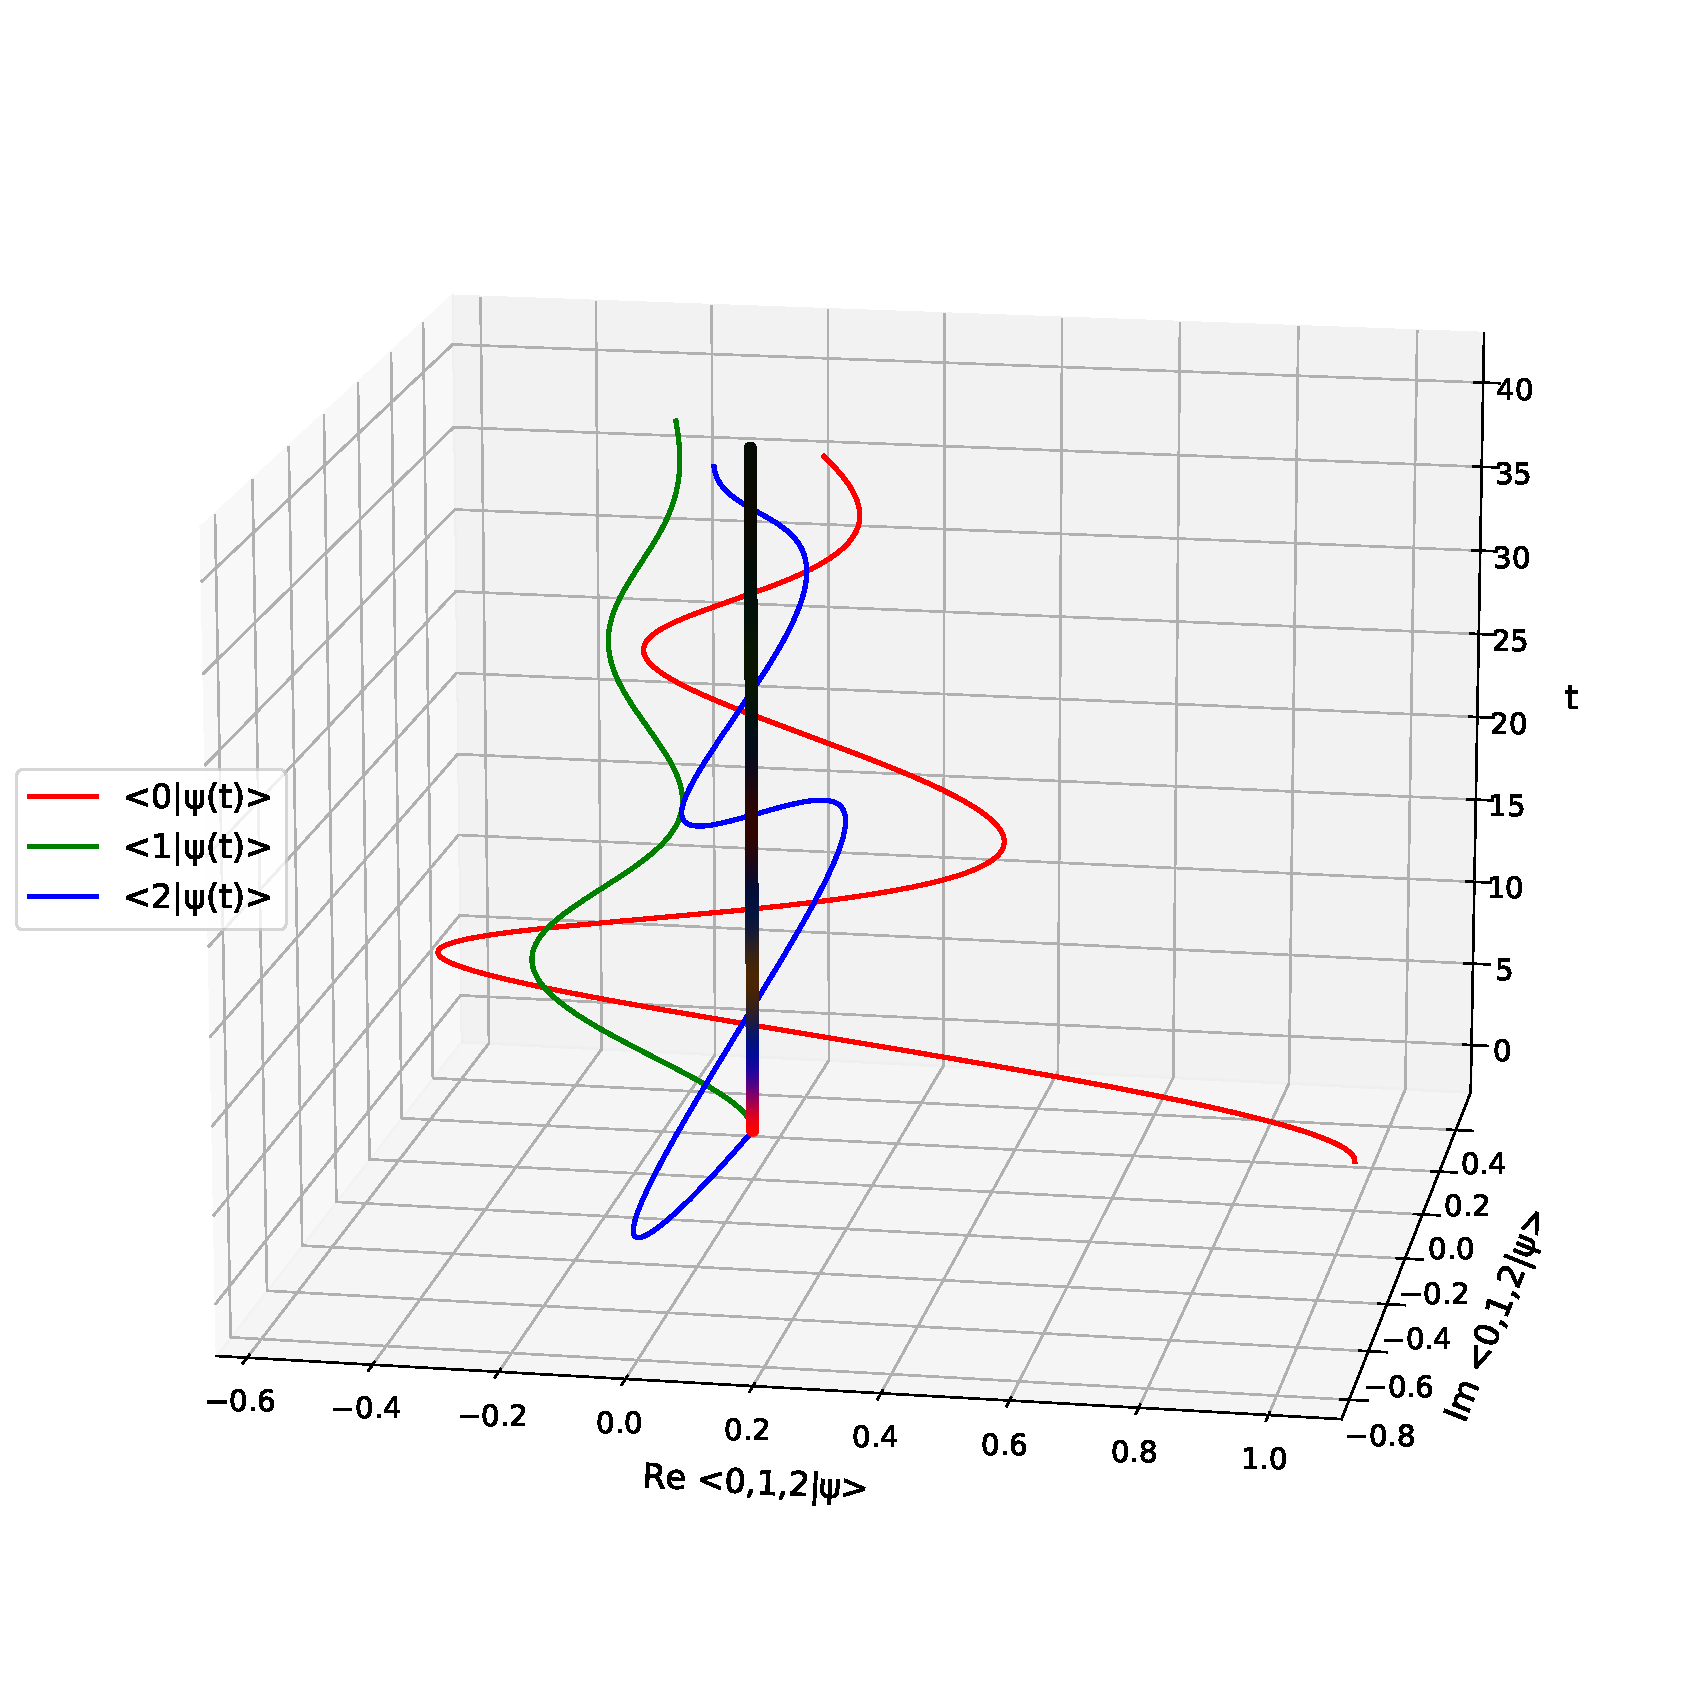
\includegraphics[height=0.41\textheight,clip,trim=0 90 40 140]{img/3ldetect/NonHermitianSpaceTime_side.pdf}
    \caption{``Side'' view.}
  \end{subfigure}
  \par\bigskip
  \begin{subfigure}[b]{\textwidth}
    \centering
    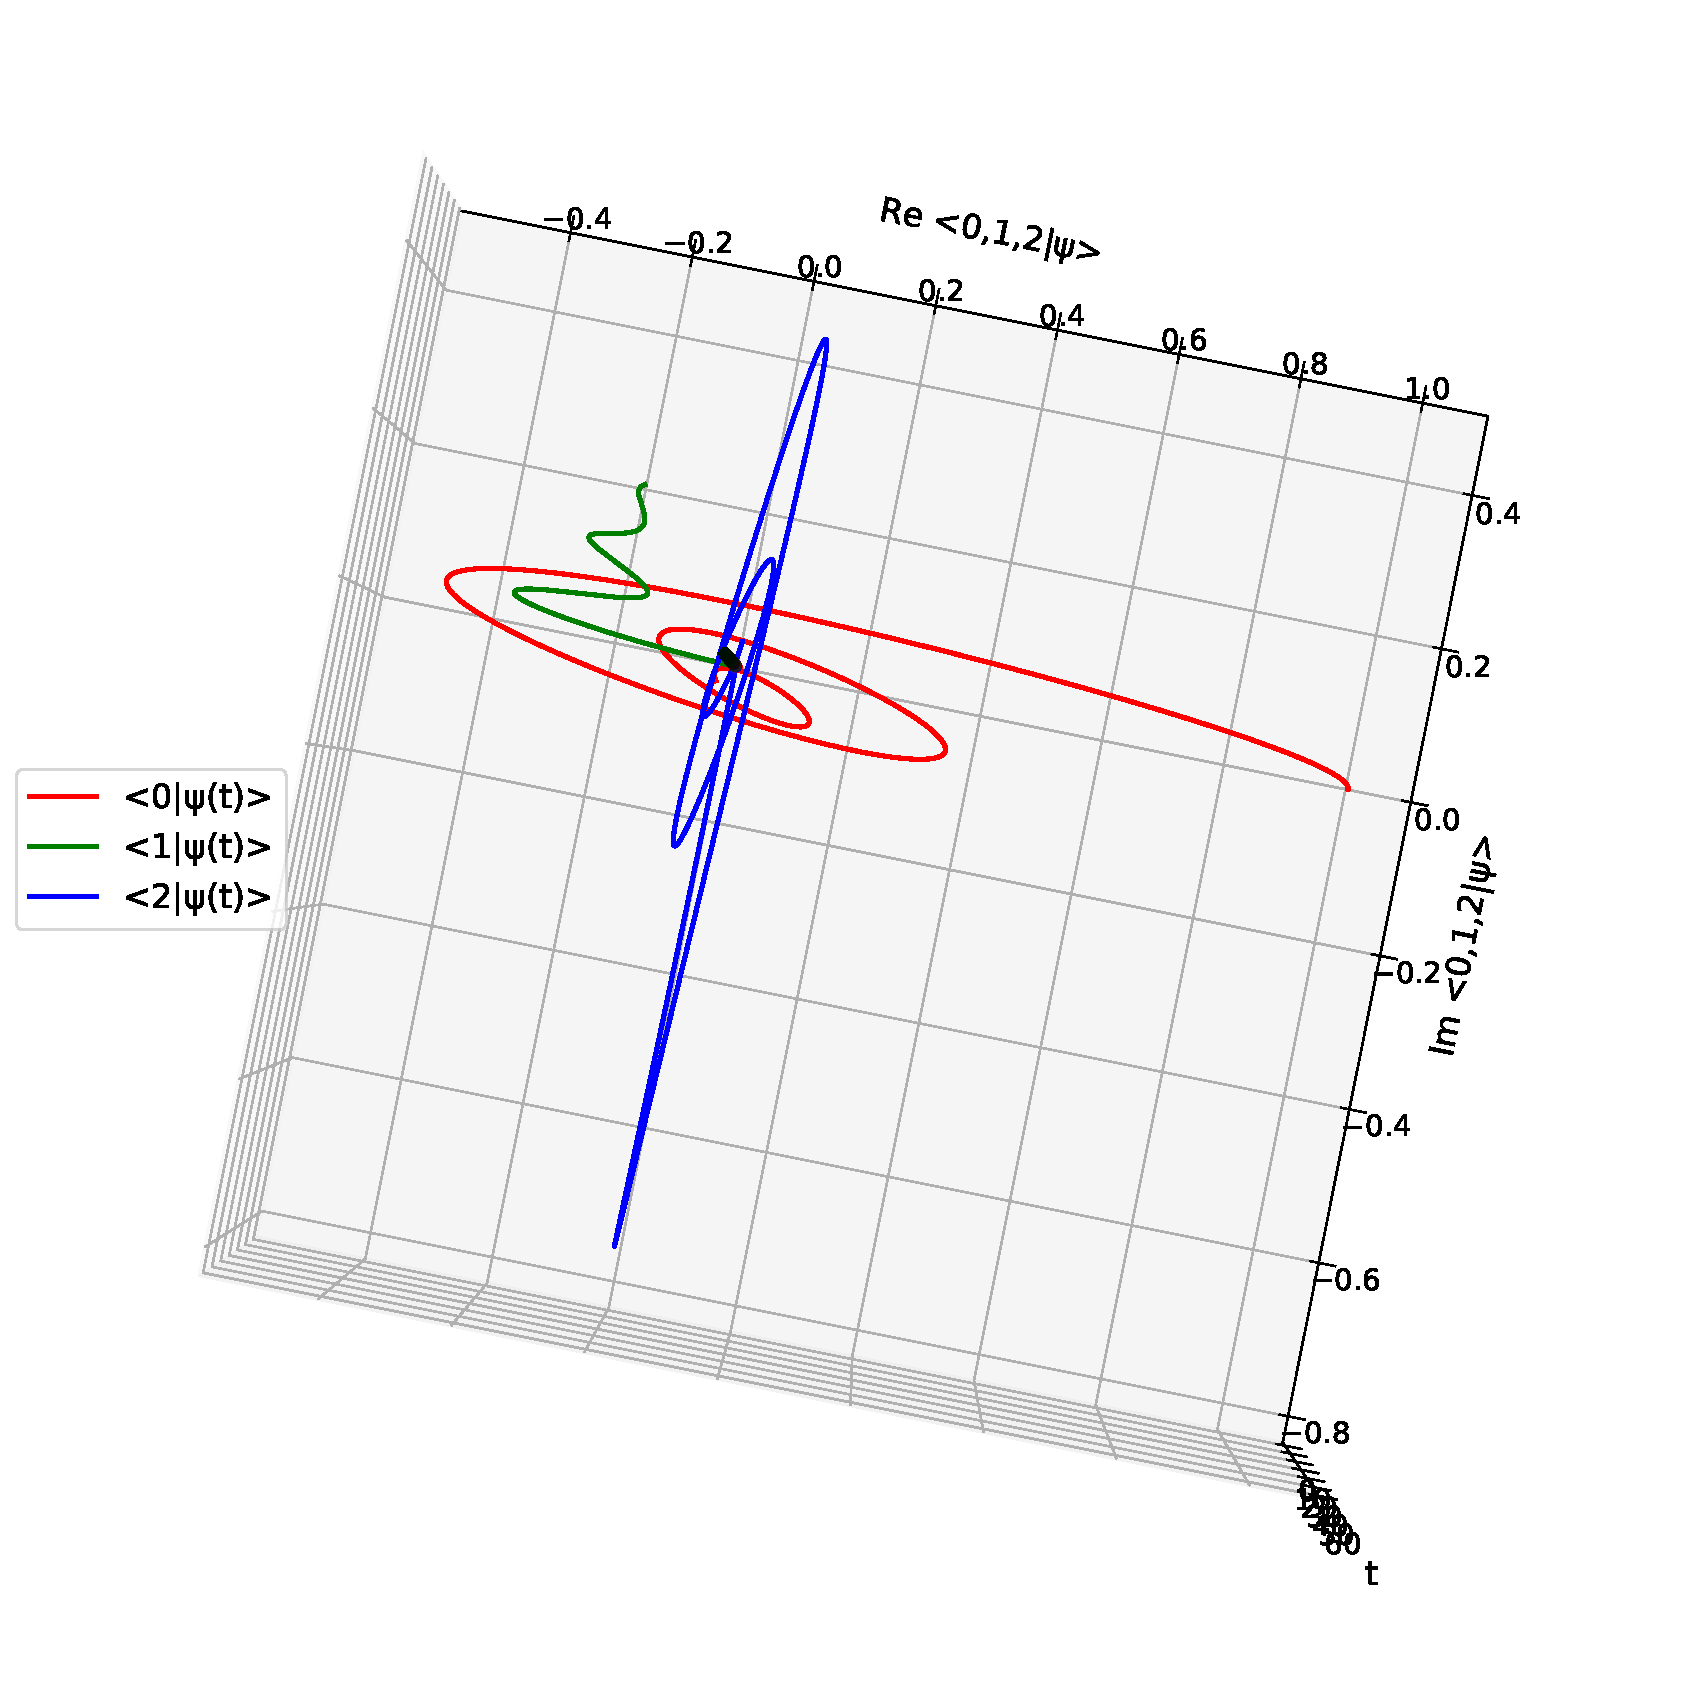
\includegraphics[height=0.44\textheight,clip,trim= 0 90 20 75]{img/3ldetect/NonHermitianSpaceTime_top.pdf}
    \caption{``Top'' view.}
  \end{subfigure}
  \caption{
    Non-Hermitian evolution: 3-D complex plot: probability amplitudes, with ``lossy''
    norm (visually, lines get closer to the time axis as $t$ increases).
  }
  \label{fig:3lev:nonHermitianEvol}
\end{figure}

According to the absorptive detector model, the loss of normalization
$-\dv{\norm{\psi}^2}{t}$ indicates the probability of detection
with respect to time, in other words: the time-of-arrival
probability distribution. It is plotted in Fig. \ref{fig:3lev:loss}.

The same results
about probabilities and normalization loss
are plotted
over a longer time interval
in Fig.~\ref{fig:3lev:nonHermitianProbs_ext}.
By comparing the latter,
back with Fig.~\ref{fig:3lev:probs:stack},
it's apparent that in the unitary case the system
periodically oscillates between $\ket{0}$ and $\ket{2}$
---transitioning through the intermediate level $\ket{1}$,
but with a small value of $\abs{\braket{1}{\psi(t)}}^2$.
Instead, within the non-unitary evolution, and with the chosen parameters,
the system is ``driven'' from $\ket{0}$ to $\ket{1}$ and,
after a transient oscillation between the three levels,
shows an asymptotic behavior.
The fidelity with respect to $\ket{1}$,
$\frac{\abs{\braket{1}{\psi(t)}}^2}{\norm{\psi(t)}^2}$,
evaluated numerically at $t=150$ is given by
\begin{lstlisting}[language=Python]
# Pick the last value of time
times_extended[-1]
\end{lstlisting}
\begin{lstlisting}
150.0
\end{lstlisting}
\begin{lstlisting}[language=Python]
# Fidelity
(np.abs(evolution_extended[1])**2)[-1] / norms_extended[-1]**2
\end{lstlisting}
The result is about $94\%$.
\begin{lstlisting}
0.9414855990054901
\end{lstlisting}
It's also worth noting that the norm does not fully vanish with $t \rightarrow +\infty$,
meaning there is a finite probabilty that detection (or ``absorption'', or spontaneous decay) never happens:
\begin{equation*}
  P_{\mathrm{nd}} = \lim_{t \rightarrow +\infty} 1 - \norm{\psi(t)}^2 \text{.}
\end{equation*}
At the ``large'' value of $t=150$ of our numerical computation, this yields
\begin{lstlisting}[language=Python]
norms_extended[-1]**2
\end{lstlisting}
\begin{lstlisting}
0.05684539507975811
\end{lstlisting}
i.e. roughly 6\% of non-absorption probabilty.
%
\begin{figure}[h]
  \begin{subfigure}[b]{\textwidth}
    \centering
    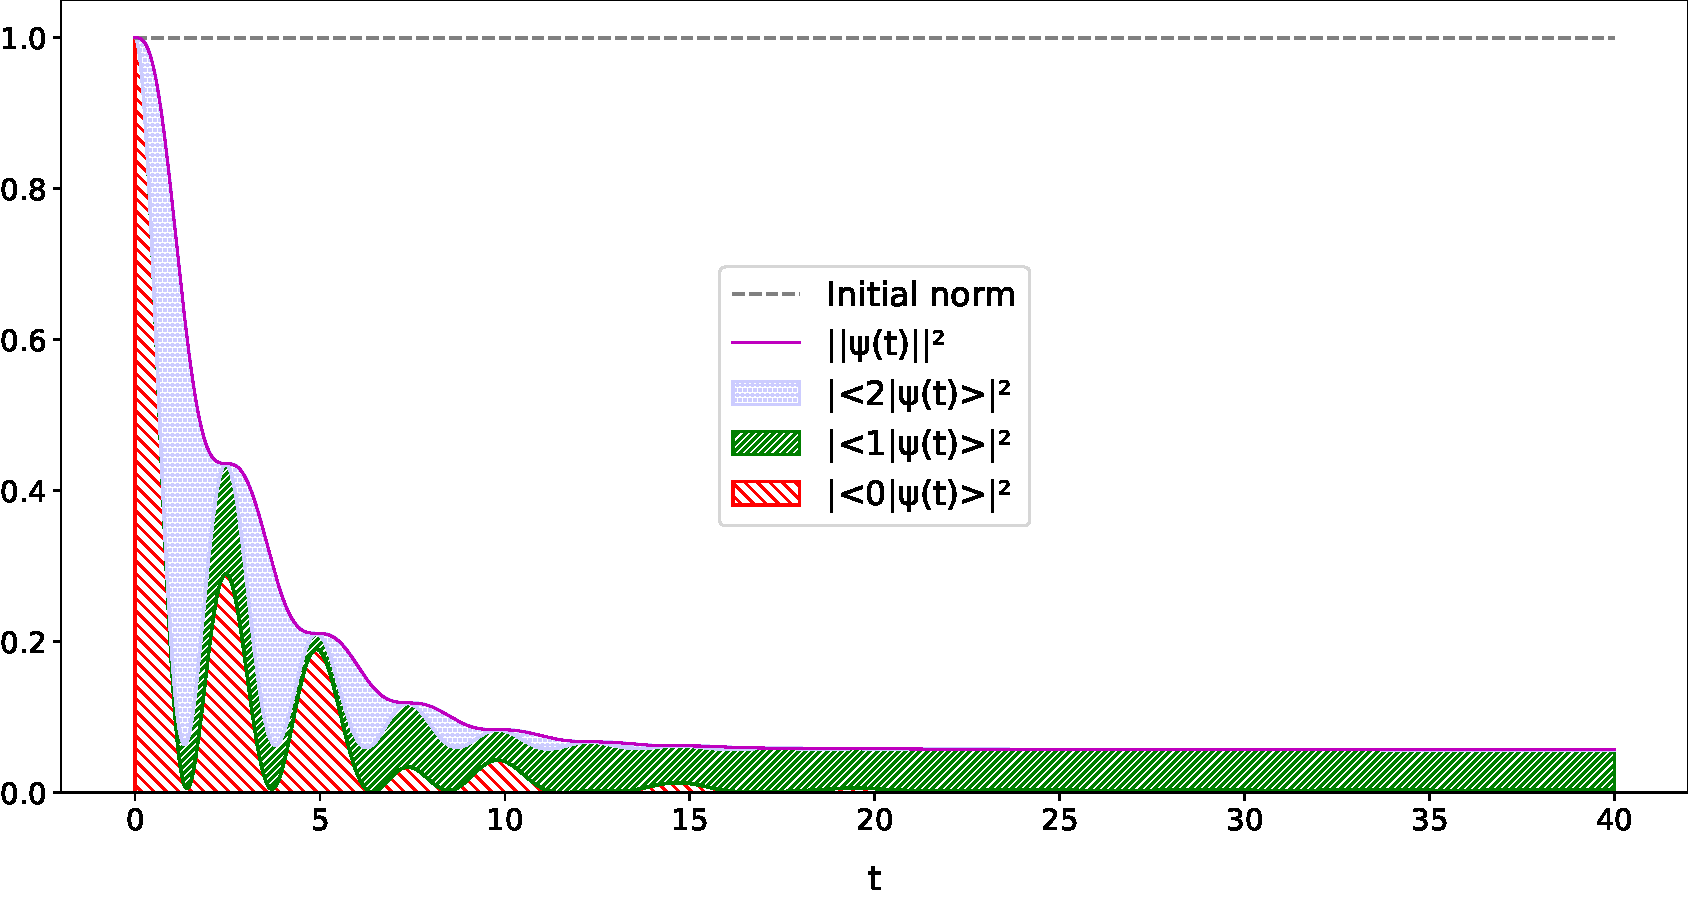
\includegraphics[width=\textwidth]{img/3ldetect/loss3color_ext.pdf}
    \subcaption{
      Probabilities and normalization loss.
    }
    \label{fig:3lev:loss3color_ext}
  \end{subfigure}
  \par\bigskip
  \par\bigskip
  \begin{subfigure}[b]{\textwidth}
    \centering
    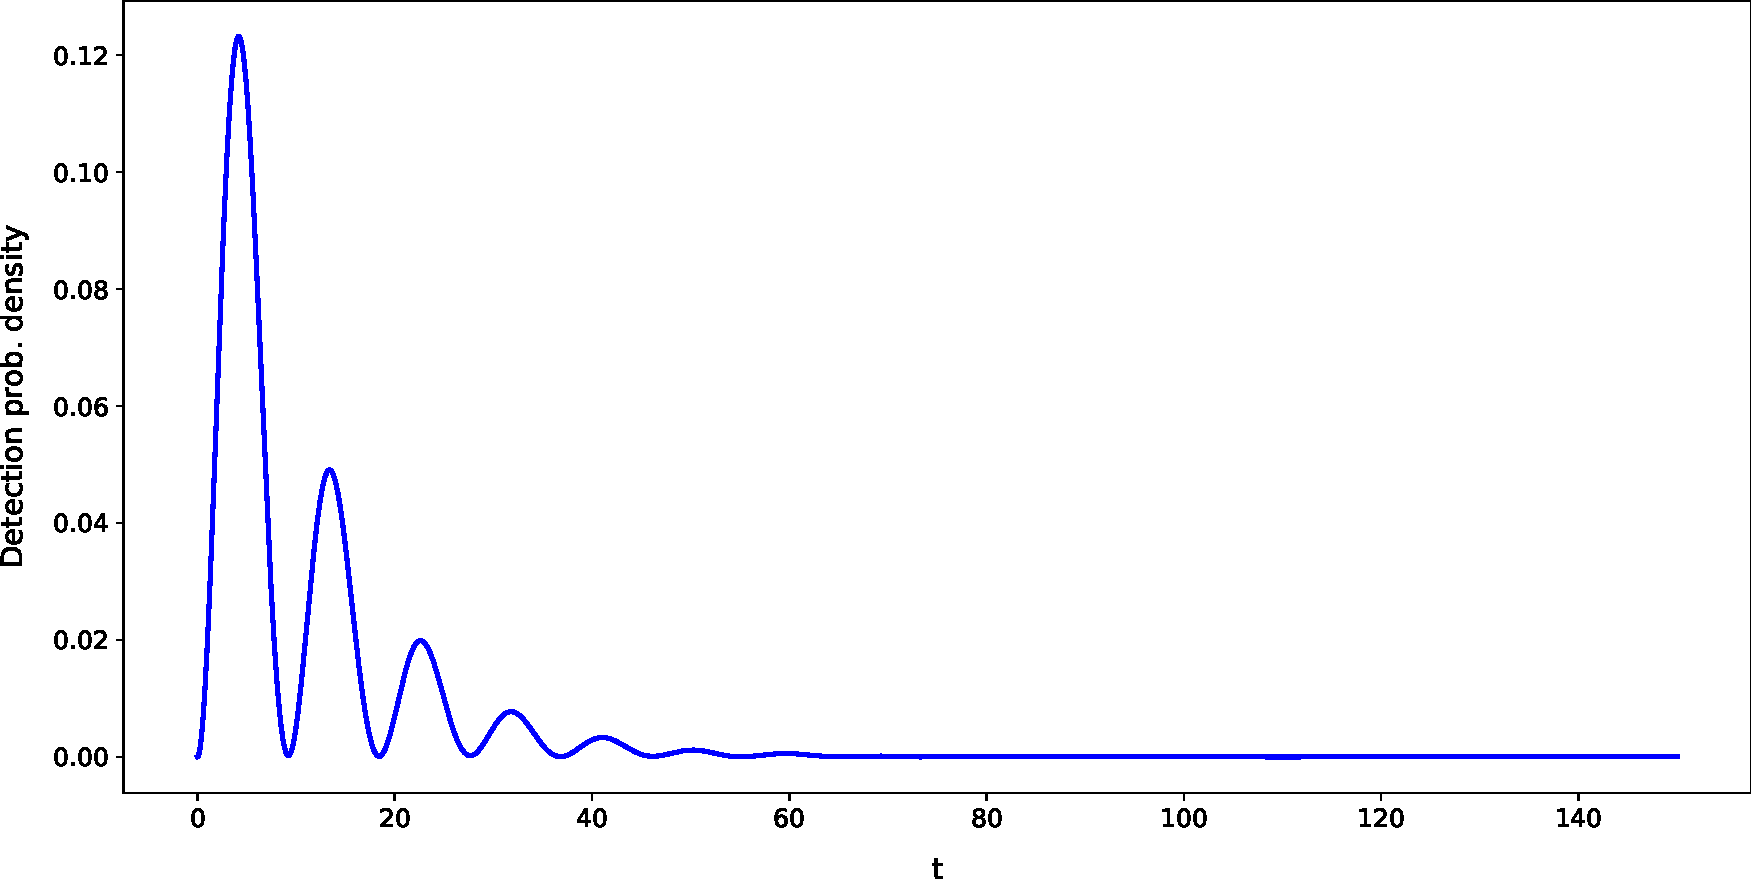
\includegraphics[width=\textwidth]{img/3ldetect/loss_ext.pdf}
    \subcaption{
      Normalization loss rate, or time-of-arrival probability distribution.
    }
    \label{fig:3lev:loss_ext}
  \end{subfigure}
  \par\bigskip
  \par\bigskip
  \caption{
    Absorptive detector model: same results as in Fig.~\ref{fig:3lev:nonHermitianProbs},
    over a longer time interval.
  }
  \label{fig:3lev:nonHermitianProbs_ext}
\end{figure}

\subsection{Discrete Page--Wootters}

Let us consider a Page--Wootters \emph{discrete} clock, with $N_{T}$ levels,
where we choose $N_{T} = 60$
(somehow resembling the 60 ticks indicating minutes or seconds
in a conventional clock\footnote{
  For a suggestive depiction, the reader may want to look at \cite[Fig.~1]{QClockPic},
  where the quantum levels of the clock are $N_{T} = 12$
  ---please note, however, that the paper allows for the clock
  and the remaining system to \emph{interact}, whereas, in the original formulation
  of the Page--Wootters mechanism,
  they are only \emph{entangled}.
}).

A basis of $\hilb{H}_T$ is chosen where the time operator $\hat{T}$ is diagonal:
\begin{equation}
  \hat{T} \repr \frac{\Delta T}{N_T} \mqty(
                                          0       &0      &\ldots &0        \\
                                          0       &1      &\ldots &0        \\
                                          \vdots  &\vdots &\ddots &\vdots   \\
                                          0       &0      &\ldots &N_{T}-1
                                        ) \text{,}
\end{equation}
where $\Delta T$ if the time interval under study.
And the frequency operator $\hat{\Omega}$ is computed via \term{Discrete Fourier Transform (DFT)}:
\begin{equation}
  \hat{\Omega} = \frac{2\pi N_T}{\Delta{T}^2} F \hat{T} F \text{.}
\end{equation}
Please note different library implementations use different conventions and definitions
of the discrete Fourier matrix,
thus
requiring appropriate factors in the relation between $\hat{T}$ and $\hat{\Omega}$.
In our code:
\begin{lstlisting}[language=Python]
# [...]
TMIN, TMAX = 0, 40
TMIN_N, TMAX_N = float(TMIN), float(TMAX)

# [...]
from scipy.linalg import dft, norm, expm, det, inv

# [...]
# Number of levels of the clock aka dimension of Time Hilbert space
NT = 60

# Time interval under study
DT = TMAX_N  # assume we start with time 0

# Time operator
T = DT * np.diag(np.arange(NT)) / NT

# Discrete Fourier
F = dft(NT, scale='sqrtn').conj()
F_dagger = F.conj().T

# Frequency operator
Omega = F @ T @ F_dagger * 2*np.pi * NT / DT**2
\end{lstlisting}

Then the ``Hamiltonian'' ${\mathbb{J}}$, acting on $\pwspace$, and defined in eq.~\eqref{eq:pwHamiltonian:nonUnitary}
is derived, with eigenvalues and eigenvectors::
\begin{lstlisting}[language=Python]
J = np.kron(Omega, np.eye(3)) + np.kron(np.eye(NT), K())
 
eigenvalues, eigenvectors = np.linalg.eig(J)
eigenvectors = eigenvectors.T
\end{lstlisting}
where the Python function \verb|K()| is the non-Hermitian operator $K$ of eq.~\eqref{eq:3lev:nonUnitaryH}.

Eigenvectors need to be ``initially normalized in $\hilb{H}_S$'' in the sense that\\
$\norm{\psi(0)}^2=1$ or,
 in Page--Wootters terms, $\langle\langle \Psi | 0 \rangle_{T}\langle 0 | \Psi \rangle \rangle = 1$.
\begin{lstlisting}[language=Python]
eigenvectors_normalized_in_S = np.empty((NT*NS, NT*NS), dtype=complex)
for i in range(NT*NS):
    eigenvectors_normalized_in_S[i] = eigenvectors[i] / norm(eigenvectors[i][:3])
\end{lstlisting}

Similarly to what illustrated in eq.~\eqref{eq:pw-vs-qm} ---and Sec.~\ref{sec:qubit:pw-vs-qm} in general---
a ``phase correction'' may be needed in order to allow a comparison with
the time evolution predicted with ``standard'' quantum mechanics
(although, still, with a non-Hermitian Hamiltonian, or \emph{complex potential}).
As the initial time is $t_0=0$ in the current example, only the
correction related to non-zero eigenvalues is required.
It's worth recalling that,
as the Wheeler-DeWitt equation reads $\mathbb{J} \dket{\Psi} = 0$,
eigenvectors of $\mathbb{J}$ related to eigenvalues ---say, $\epsilon_{i}$---
which are not zero,
need to be corrected by ``rigidly shifting the spectrum of $H_{S}$
by [$\epsilon_{i}$]'' (once again, \cite[``\textit{The Zero-eigenvalue}'']{Lloyd:Time}):
\begin{equation}
  \dket{\epsilon_i} \;\longrightarrow\; \dket{\Phi_{i}} \eqbydef e^{ -\iu \hat{T} \epsilon_{i} \, \ox \, \idop_{S}} \dket{\epsilon_{i}} \text{,}
  \label{eq:3lev:correction}
\end{equation}
where it has been set $\hbar=1$. This translates in code as follows:\footnote{
  In the Python code, \Verb+i+ is an iteration index and \Verb|1j| is the imaginary unit
  (the latter is a convention of the language).
  In eq.\eqref{eq:3lev:correction},
  $i$ is a summation index and $\iu$ (upright typeface) is the imaginary unit.
  The context may also help in interpreting the notation correctly.
}
\begin{lstlisting}[language=Python]
histories = np.empty((NT*NS, NT*NS), dtype=complex)

for i in range(NT*NS):
    histories[i] = \
        expm(np.kron( -1j*T*eigenvalues[i], np.eye(NS) )) @ \
        eigenvectors_normalized_in_S[i]
\end{lstlisting}
%
With a slightly different notation,
the \Verb|histories[i]|
correspond to the $\dket{\Phi_i}$ in Eq.~\eqref{eq:3lev:correction}.
They are named \Verb!histories! because each of them
(and any linear combination, per quantum superposition principle)
encodes a possible evolution (altough with discrete time resolution)
of the system along the whole time interval $[0, \Delta T]$.

A comparison can be made, in principle, between the quantities
\begin{equation}
  x \sim x
\end{equation}

%%%%%%%%%%%%%%%%%%%%%%%%%%%%%%%%%%%%%%%%%%%%%%%%%%%%%%%%%%%%%%%%%%%%%%%

%%
%%
%%
%%

% P-W

\begin{figure}[h]
  \begin{subfigure}[b]{\textwidth}
    \centering
    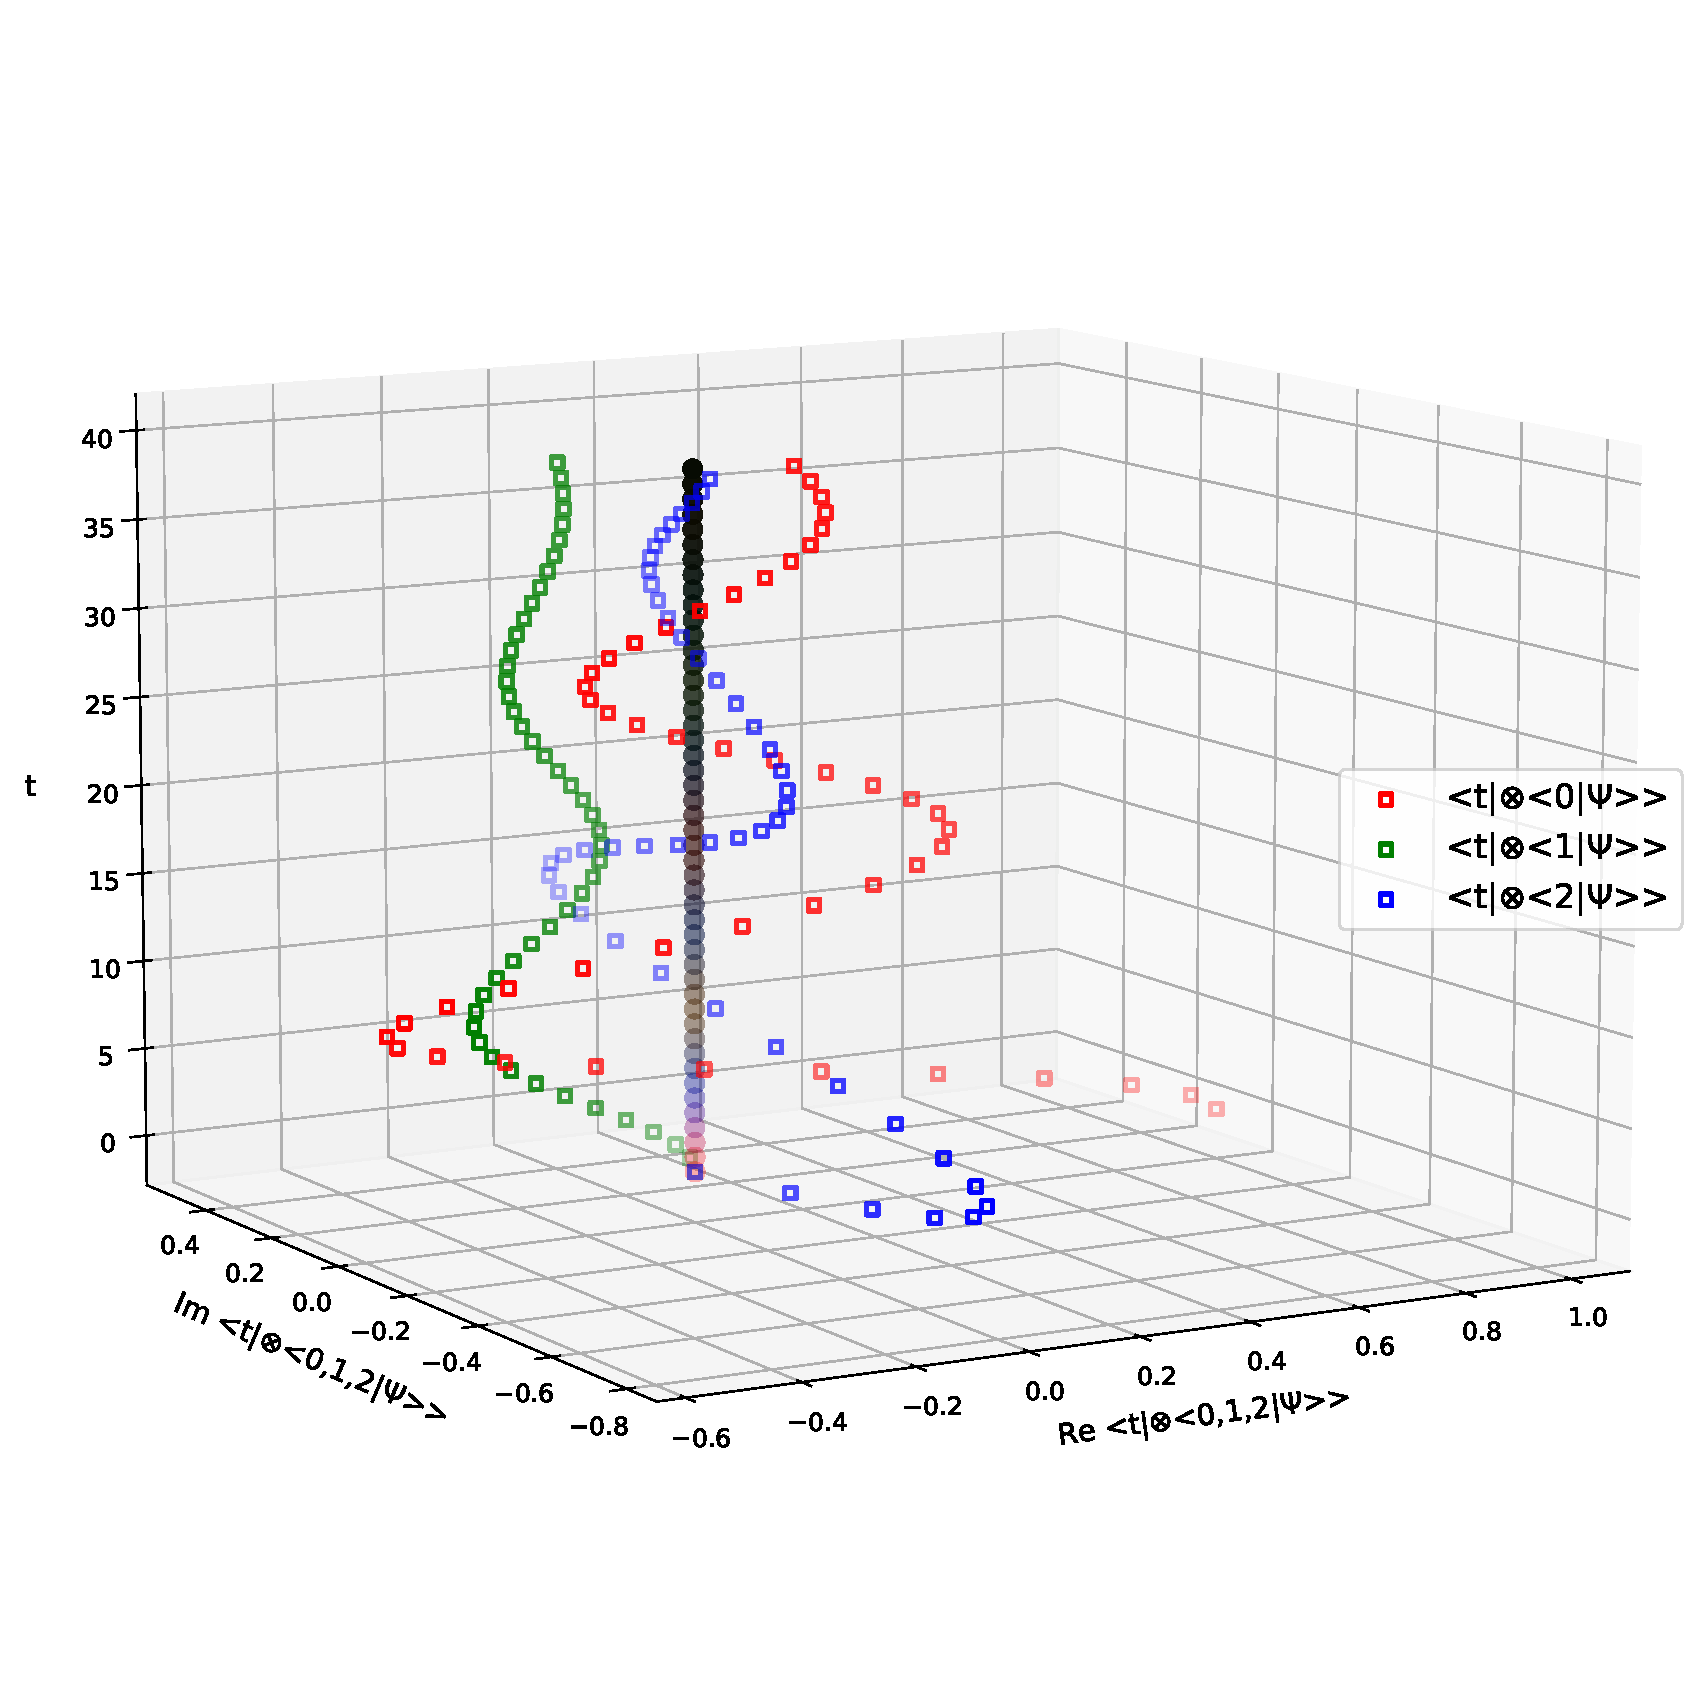
\includegraphics[height=0.41\textheight,clip,trim=0 90 0 140]{img/3ldetect/PWSpaceTime_side.pdf}
    \caption{Foo.}
  \end{subfigure}
  \par\bigskip
  \begin{subfigure}[b]{\textwidth}
    \centering
    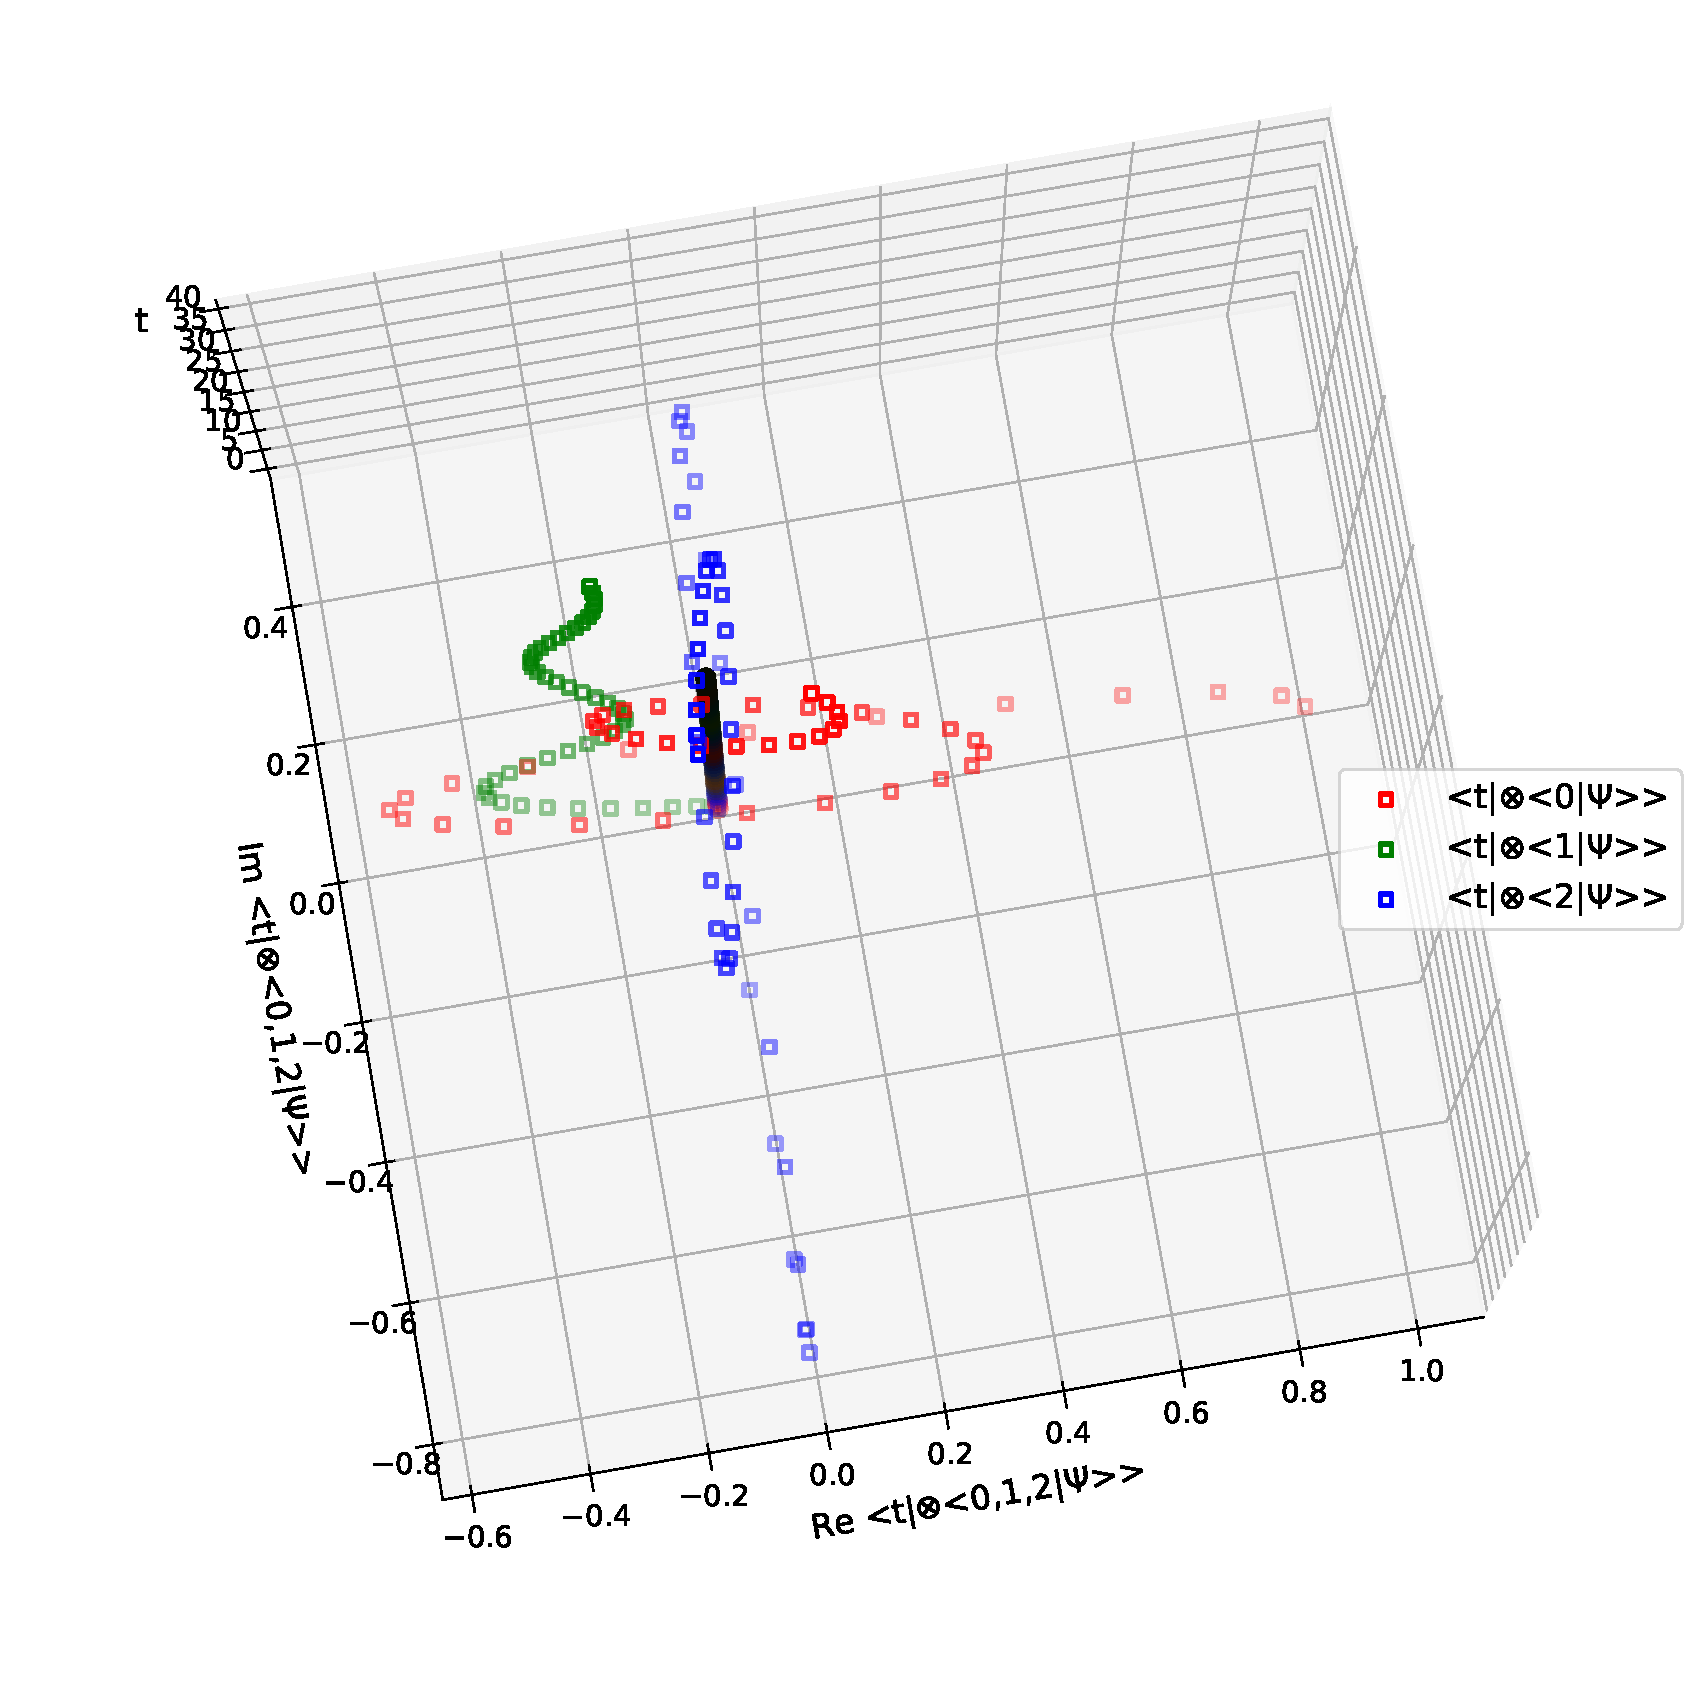
\includegraphics[height=0.48\textheight,clip,trim= 0 60 0 100]{img/3ldetect/PWSpaceTime_top.pdf}
    \caption{Bar.}
  \end{subfigure}
  \caption{FooBar.}
  %\label{fig:psi_V}
\end{figure}

% P-W vs QM


\begin{figure}[]
  \centering
  \begin{subfigure}{\textwidth}
      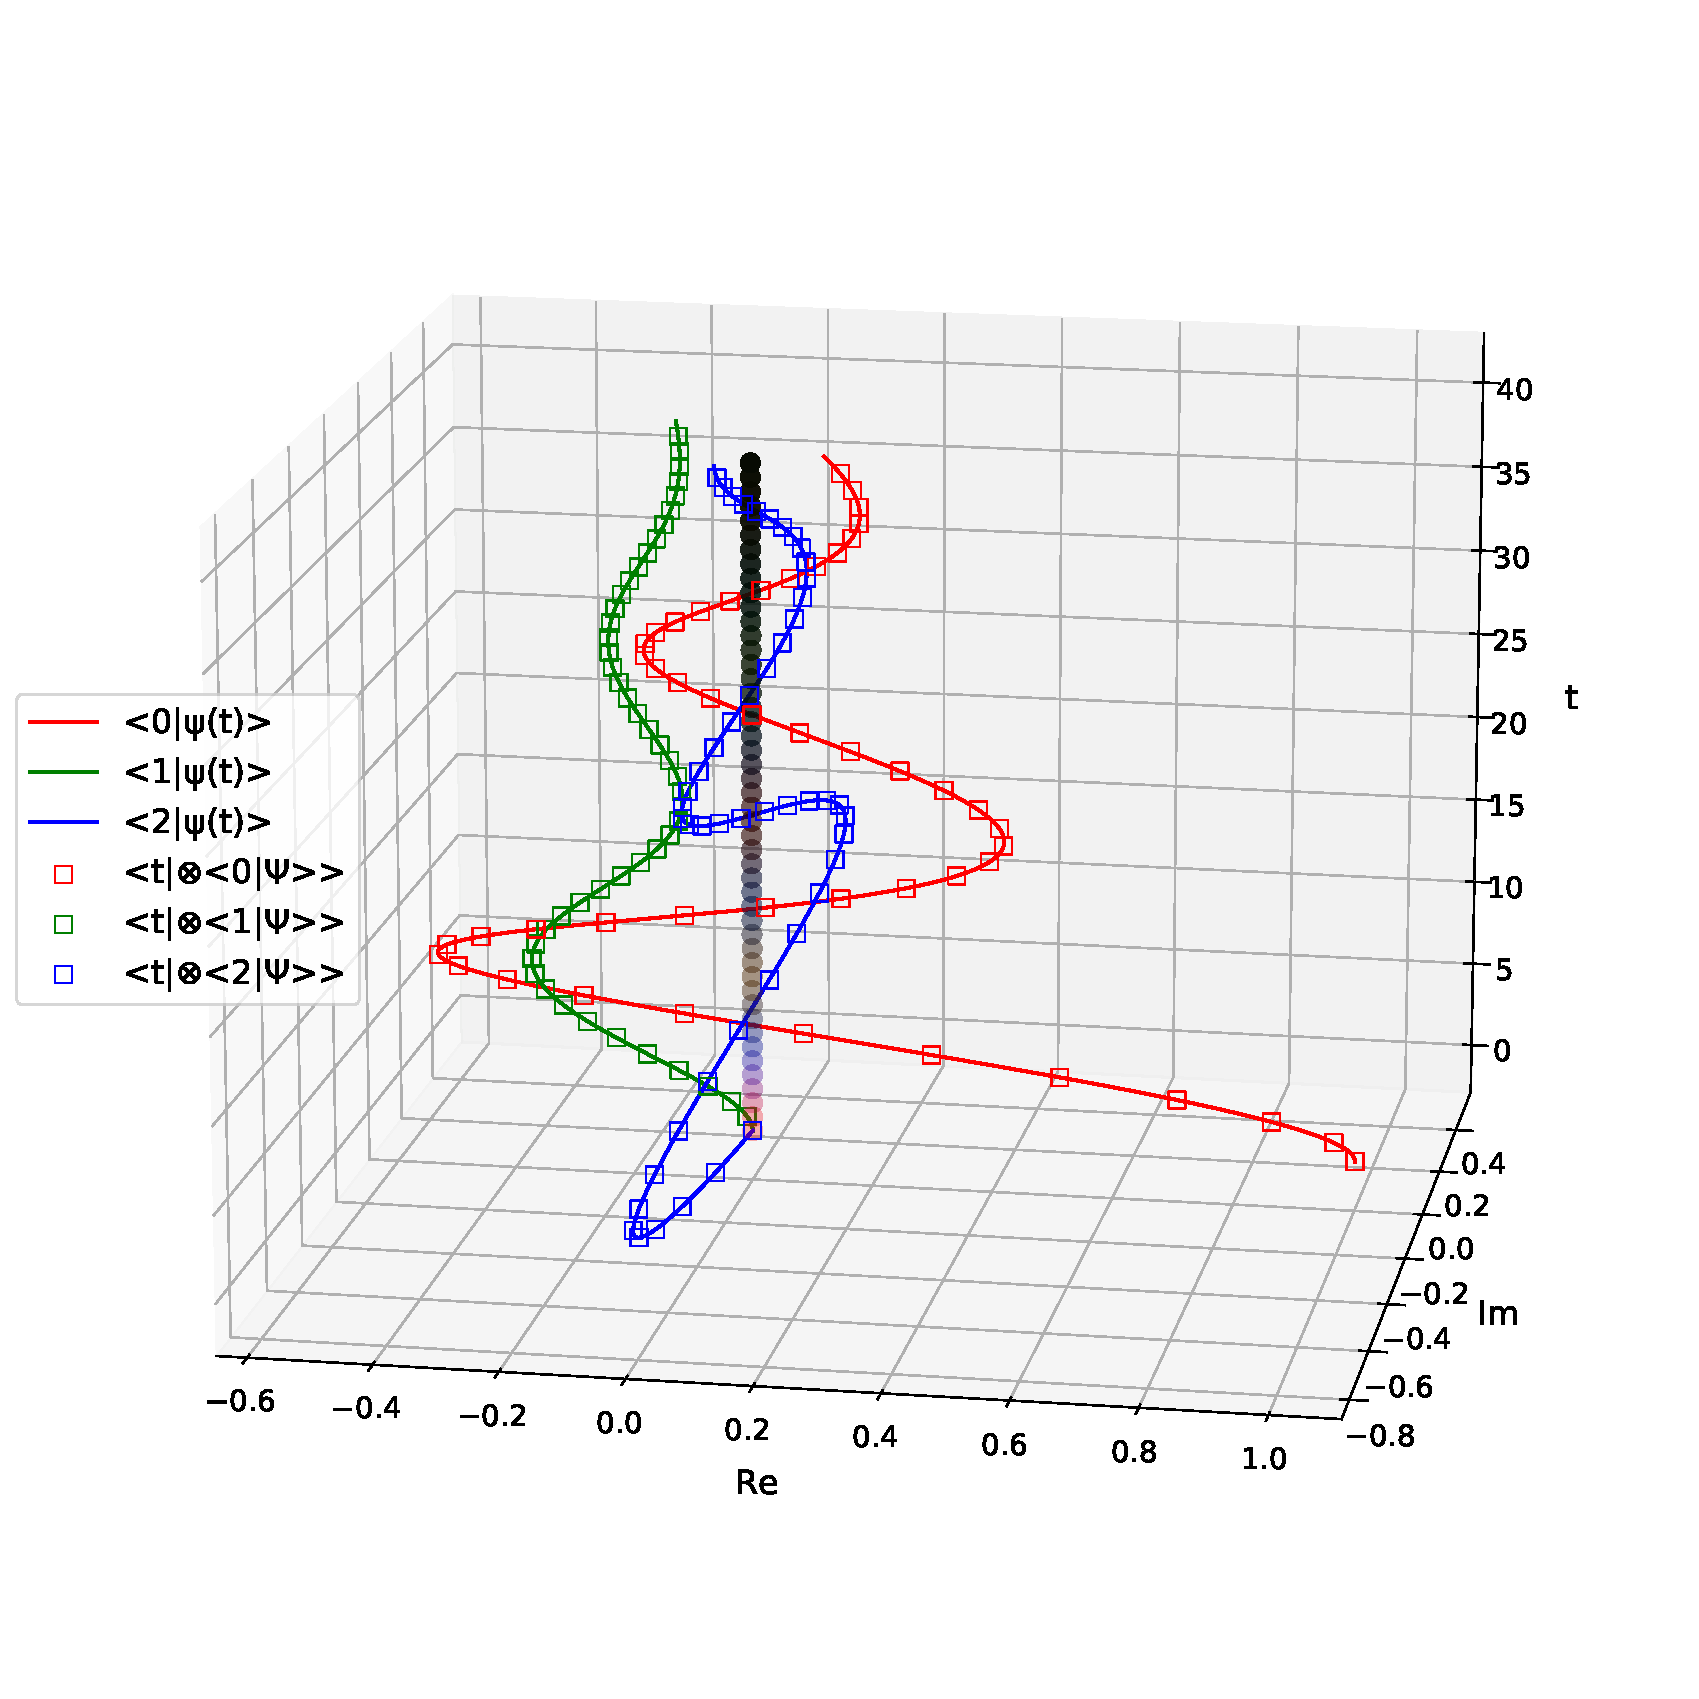
\includegraphics[width=\textwidth]{img/3ldetect/PWSpaceTimeFit_side.pdf}
      \subcaption{Foo.}
      %\label{fig:arm1}
  \end{subfigure}
  \caption{Foobar.}
\end{figure}
\begin{figure}\ContinuedFloat
  \centering
  \begin{subfigure}{\textwidth}
      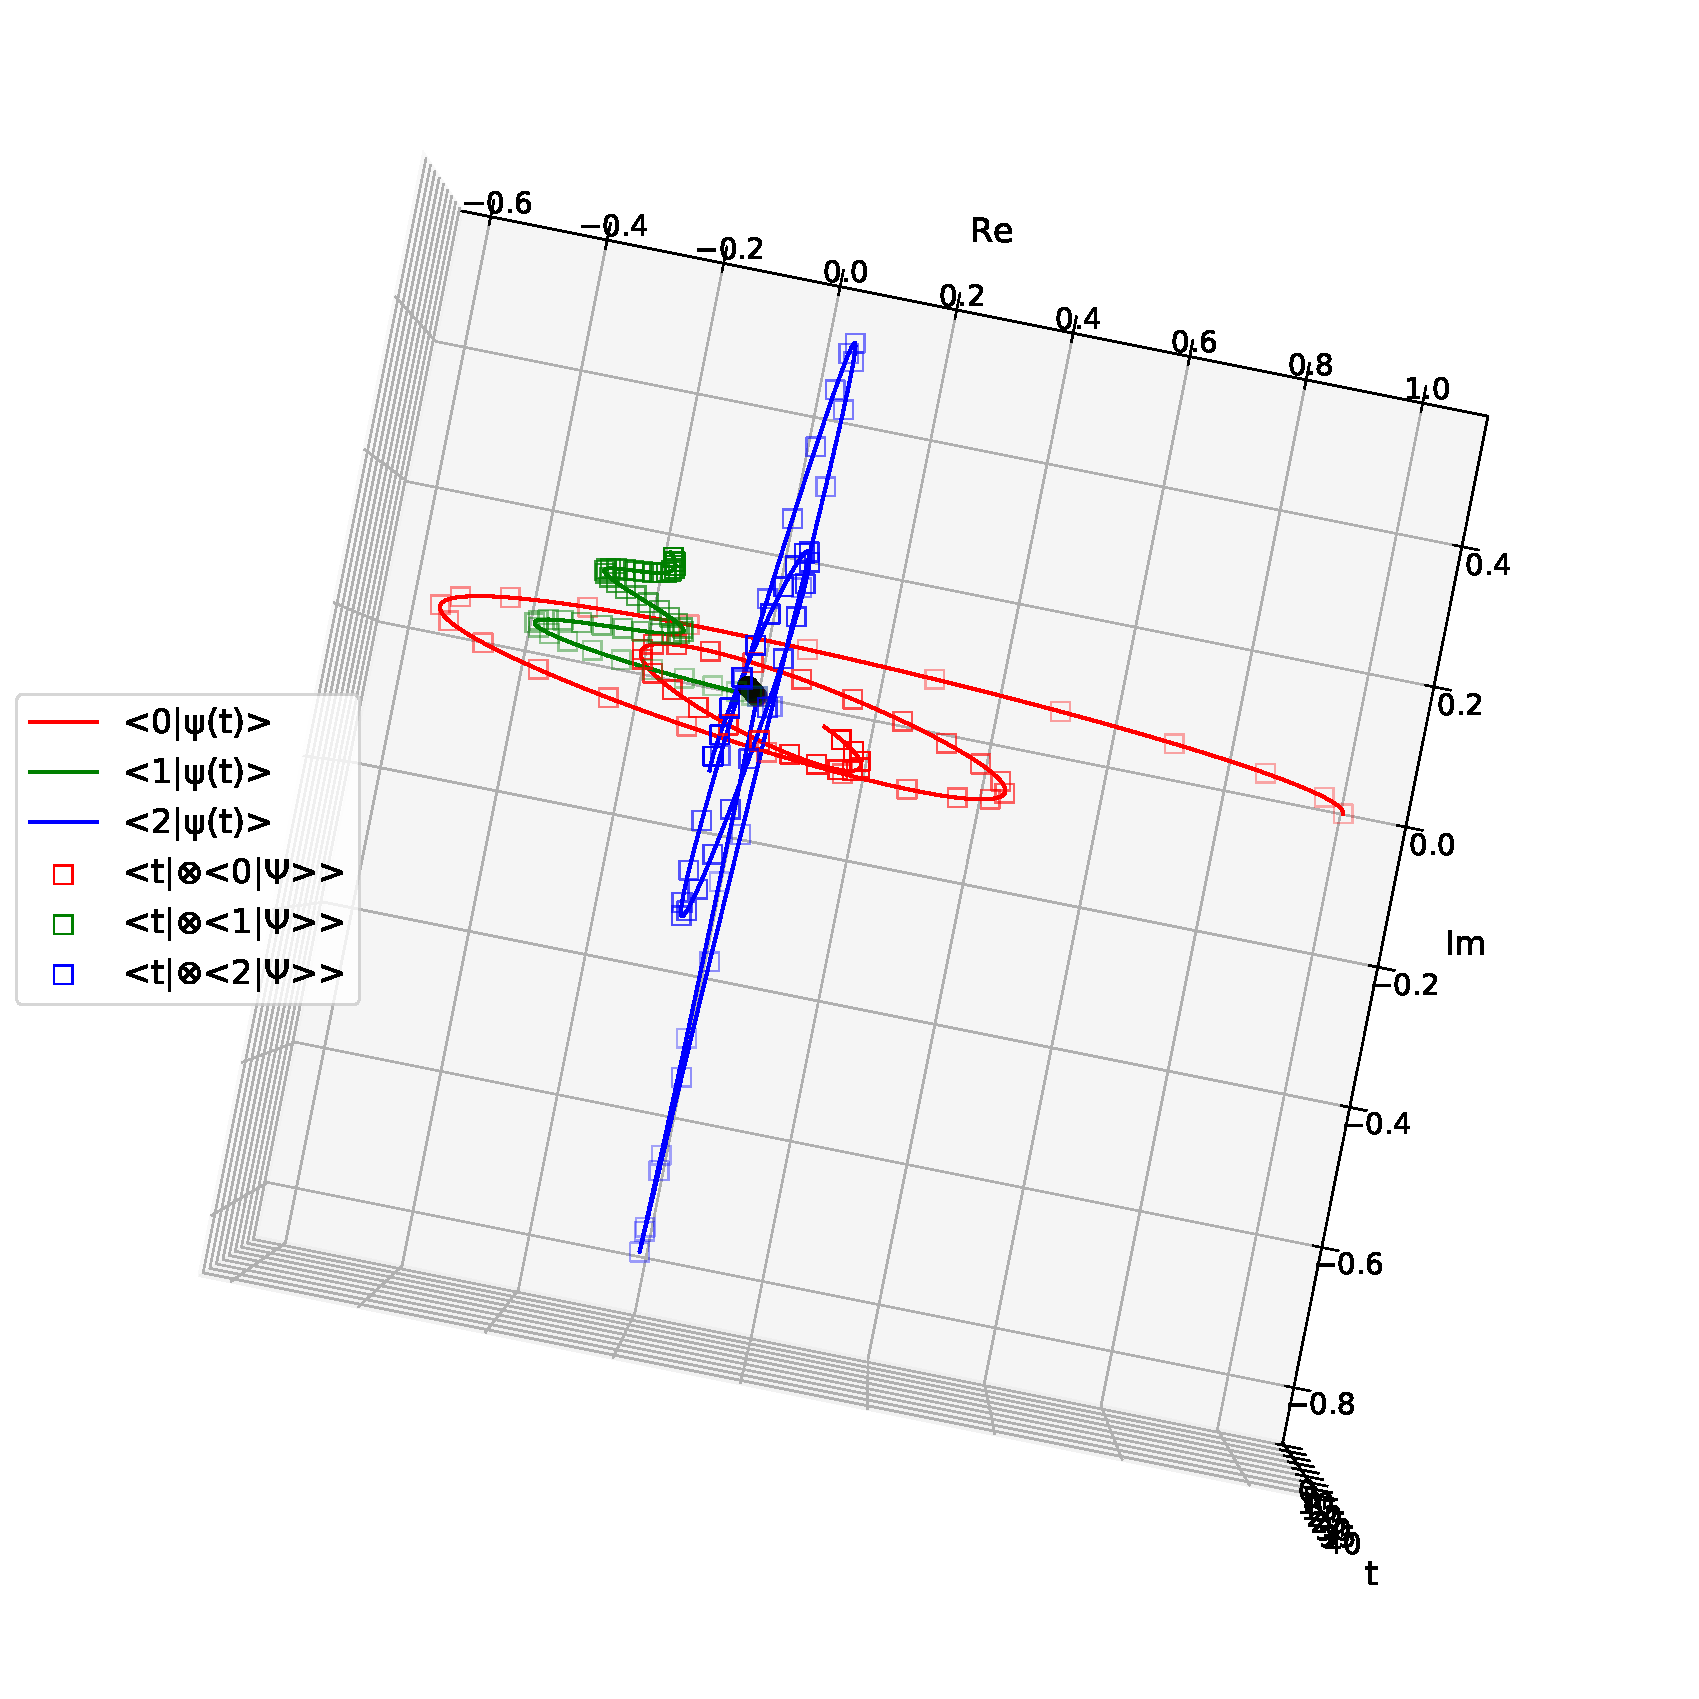
\includegraphics[width=\textwidth]{img/3ldetect/PWSpaceTimeFit_top.pdf}
      \subcaption{Bar.}
      %\label{fig:arm3}
  \end{subfigure}
  \caption{Foobar (cont.)}
\end{figure}

% P-W (bayesian) vs Detector model (norm. loss, Allcock...) detection probability

\begin{figure}[h!]
  \centering
  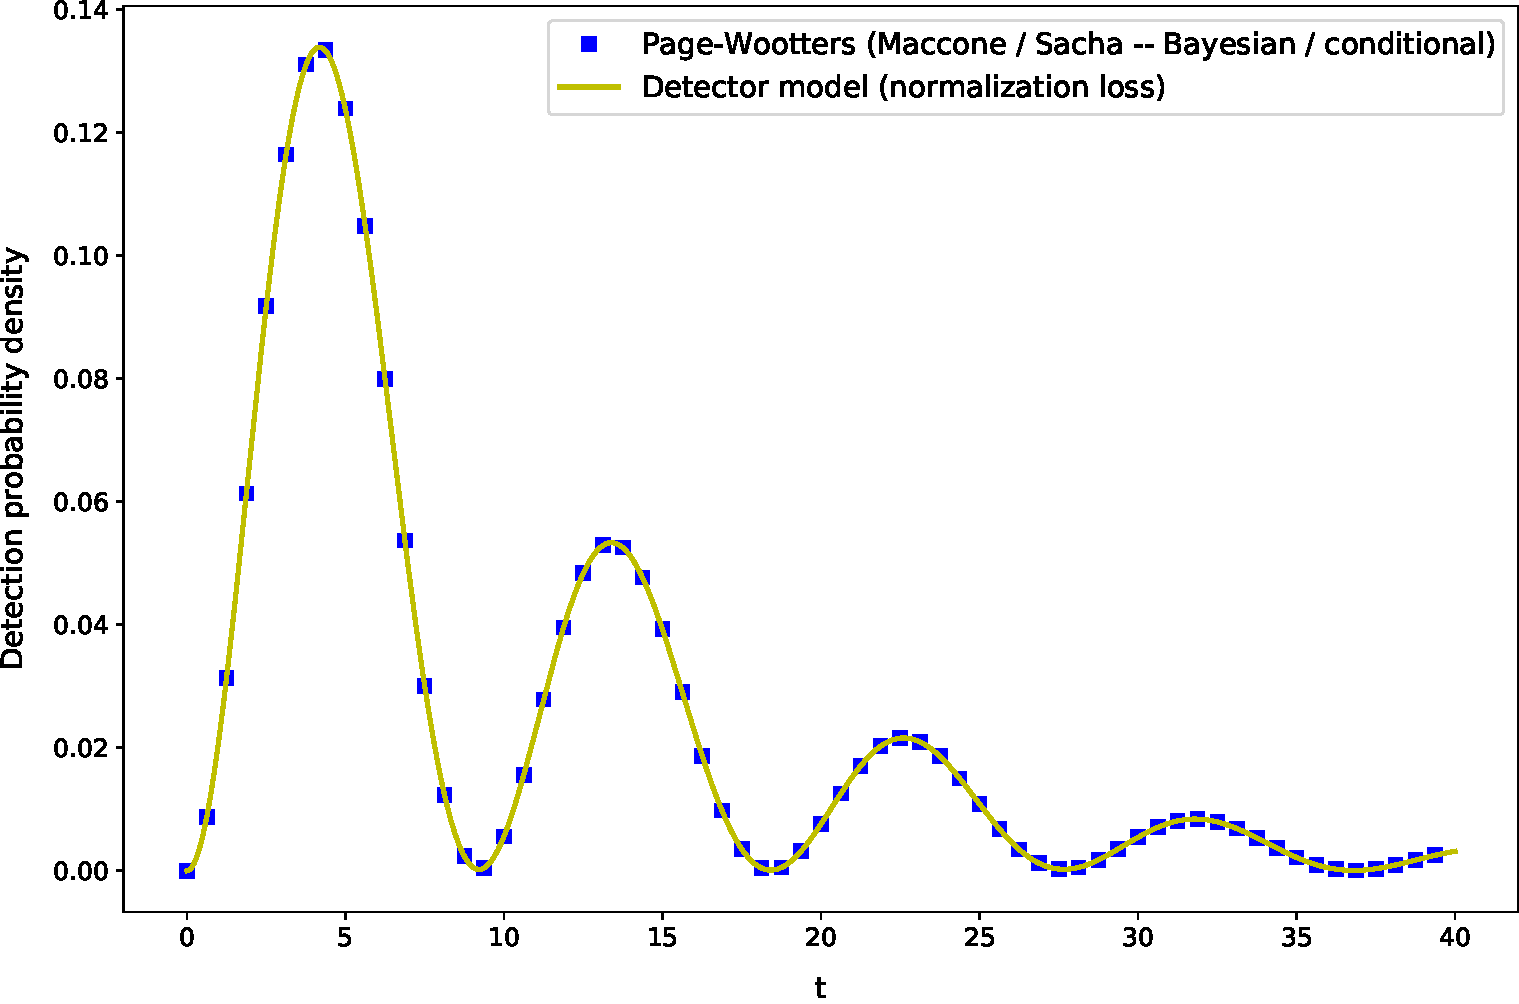
\includegraphics[width=\textwidth]{img/3ldetect/conditionalProbFit.pdf}
  \caption{Foo.}
  %\label{fig:psi_V}
\end{figure}